\documentclass[10pt,letterpaper,oneside,twocolumn,journal]{IEEEtran}

% 
% 8888888 888b     d888 8888888b.   .d88888b.  8888888b. 88888888888 .d8888b.  
%   888   8888b   d8888 888   Y88b d88P" "Y88b 888   Y88b    888    d88P  Y88b 
%   888   88888b.d88888 888    888 888     888 888    888    888    Y88b.      
%   888   888Y88888P888 888   d88P 888     888 888   d88P    888     "Y888b.   
%   888   888 Y888P 888 8888888P"  888     888 8888888P"     888        "Y88b. 
%   888   888  Y8P  888 888        888     888 888 T88b      888          "888 
%   888   888   "   888 888        Y88b. .d88P 888  T88b     888    Y88b  d88P 
% 8888888 888       888 888         "Y88888P"  888   T88b    888     "Y8888P"  
%                                                                              
%                                                                              
%                                                                              
% 

% Graphics
\usepackage{tikz}
\usepackage{graphicx}
% Maths
\usepackage{amsmath}
\usepackage{amsfonts}
\usepackage{amsthm}
\usepackage{mathtools}
\usepackage{bm}
% Algorithms
\usepackage{algorithm}
\usepackage{algpseudocode}
% Local
\usepackage{ISASmacros/isasmathmacros}
% Equal last columns
\usepackage{flushend}

% Environments
\theoremstyle{definition}
\newtheorem{definition}{Definition}[section]

\theoremstyle{definition}
\newtheorem{theorem}{Theorem}[section]

\theoremstyle{remark}
\newtheorem*{remark}{Remark}

% Algorithm settings
\algnewcommand{\LineComment}[1]{\State \(\triangleright\) #1}

% Tikz settings
\usetikzlibrary{math}

% Tikz reused commands
\tikzset{
   plane/.pic = {
    \draw[fill]  plot[smooth, tension=0.6] coordinates {
        (-0.65,-0.9) 
        (-0.6,-0.85) 
        (-0.4,-0.75) 
        (-0.25,-0.65) 
        (-0.15,-0.5) 
        (-0.12,-0.3) 
        (-0.1,-0.1) 
        (0,0) 
        (0.1,-0.1) 
        (0.12,-0.3) 
        (0.15,-0.5) 
        (0.25,-0.65) 
        (0.4,-0.75) 
        (0.6,-0.85) 
        (0.65,-0.9)
        } -- plot[smooth, tension=0.6] coordinates {
        (0.65,-0.9) 
        (0.15,-0.91)
        (0.35,-1.1) 
        (0.37,-1.15)
        } -- plot[smooth, tension=0.6] coordinates {
        (0.37,-1.15)
        (0,-1.12) 
        (-0.37,-1.15) 
        } -- plot[smooth, tension=0.6] coordinates {
        (-0.37,-1.15)
        (-0.35,-1.1) 
        (-0.15,-0.91) 
        (-0.65,-0.9) 
        } -- cycle;
   }
}
\definecolor{pyplotblue}{RGB}{31,119,180}
\definecolor{pyplotorange}{RGB}{255,127,14}

% Used to make a few encryption functions fit in one line
\newcommand\shrtdots{\!...}

% correct bad hyphenation here
\hyphenation{op-tical net-works semi-conduc-tor}

% Requested for submission
\pdfminorversion=4

% Start
\begin{document}

% paper title
\title{Distributed Range-Only Localisation that Preserves Sensor and Navigator Privacies}

% author names and IEEE memberships
\author{Marko~Ristic$^{1}$,
        Benjamin~Noack$^{1}$,~\IEEEmembership{Member,~IEEE,}
        and~Uwe~D.~Hanebeck$^{2}$,~\IEEEmembership{Fellow,~IEEE}% <-this % stops a space
\thanks{$^{1}$Marko Ristic and Benjamin Noack are with the Autonomous Multisensor Systems Group (AMS), Institute for Intelligent Cooperating Systems (ICS), Otto von Guericke University Magdeburg (OVGU), Germany (e-mail: \{marko.ristic, benjamin.noack\}@ovgu.de).}% <-this % stops a space
\thanks{$^{2}$Uwe D. Hanebeck is with the Intelligent Sensor-Actuator-Systems Laboratory (ISAS), Institute for Anthropomatics, Karlsruhe Institute of Technology (KIT), Germany (e-mail: uwe.hanebeck@kit.edu).}}% <-this % stops a space

% make the title area
\maketitle

% 
%        d8888 888888b.    .d8888b. 88888888888 8888888b.         d8888  .d8888b. 88888888888 
%       d88888 888  "88b  d88P  Y88b    888     888   Y88b       d88888 d88P  Y88b    888     
%      d88P888 888  .88P  Y88b.         888     888    888      d88P888 888    888    888     
%     d88P 888 8888888K.   "Y888b.      888     888   d88P     d88P 888 888           888     
%    d88P  888 888  "Y88b     "Y88b.    888     8888888P"     d88P  888 888           888     
%   d88P   888 888    888       "888    888     888 T88b     d88P   888 888    888    888     
%  d8888888888 888   d88P Y88b  d88P    888     888  T88b   d8888888888 Y88b  d88P    888     
% d88P     888 8888888P"   "Y8888P"     888     888   T88b d88P     888  "Y8888P"     888     
%                                                                                             
%                                                                                             
%                                                                                             
% 

\begin{abstract}
Distributed state estimation and localisation methods have become increasingly popular with the rise of ubiquitous computing, and have led naturally to an increased concern regarding data and estimation privacy. Traditional distributed sensor navigation methods typically involve the leakage of sensor or navigator information by communicating measurements or estimates and thus do not preserve participants’ privacy. The existing approaches that do provide such guarantees, fail to address sensor and navigator privacy in the common application of model-based range-only estimation, consequently forfeiting broad applicability. In this work, we define a notion of privacy-preserving linear combination aggregation and use it to derive a modified Extended Kalman Filter using range measurements such that navigator location, sensors' locations, and sensors' measurements are kept private during navigation. Additionally, a formal cryptographic backing is presented to guarantee our method's privacy as well as an implementation to evaluate its performance. The novel, provably secure, range-based localisation method has applications in a variety of environments where sensors may not be trusted or estimates are considered sensitive, such as autonomous vehicle localisation or air traffic navigation.
\end{abstract}

% Key words
\begin{IEEEkeywords}
State Estimation, Data Privacy, Sensor Fusion, Extended Kalman Filter.
\end{IEEEkeywords}

% Creates the second title
\IEEEpeerreviewmaketitle

% 
% 8888888 888b    888 88888888888 8888888b.   .d88888b.  
%   888   8888b   888     888     888   Y88b d88P" "Y88b 
%   888   88888b  888     888     888    888 888     888 
%   888   888Y88b 888     888     888   d88P 888     888 
%   888   888 Y88b888     888     8888888P"  888     888 
%   888   888  Y88888     888     888 T88b   888     888 
%   888   888   Y8888     888     888  T88b  Y88b. .d88P 
% 8888888 888    Y888     888     888   T88b  "Y88888P"  
%                                                        
%                                                        
%                                                        
% 

\section{Introduction} \label{sec:introduction}
\IEEEPARstart{L}{ocalisation} methods in distributed sensor environments have long been an active topic of research \cite{pierceIntroductionLoran1946,ligginsDistributedDataFusion2012,liContributedReviewSourcelocalization2016} and have characterised many advancements of Kalman and Bayesian estimation theory \cite{mutambaraDecentralizedEstimationControl1998}. In particular, range-based localisation methods, including signal strength measurements \cite{wangConvexCombinationSource2018,heRangeFreeLocalizationSchemes2003}, acoustic ranges \cite{beutlerNewNonlinearFiltering2004} and ultra-wideband ranges \cite{geziciLocalizationUltraWidebandRadios2005}, have found large application due to the prevalence of suitable sensors. In most cases, these localisation methods require the gathering of measurements centrally, where an estimate of location can be computed. With recent developments in distributed and cloud computing, uses of wireless and public communication channels for data transfer have become widespread, and the additional requirements of data privacy and state secrecy have become particularly relevant \cite{brennerSecretProgramExecution2011,renSecurityChallengesPublic2012}.

Typical cryptographic secrecy involves hiding all transferred data such that external parties in the communication network learn no new information from acquired encryptions. This can be achieved with common symmetric and public-key encryption scheme such as AES \cite{gueronIntelAdvancedEncryption2010} and RSA \cite{rivestMethodObtainingDigital1978}, respectively. In some cases however, partial data leakage or encrypted data processing is required for achieving a desired goal which has led to several homomorphic and functional encryption schemes \cite{paillierPublicKeyCryptosystemsBased1999,shiPrivacyPreservingAggregationTimeSeries2011,joyeScalableSchemePrivacyPreserving2013,chotardDecentralizedMultiClientFunctional2018} finding uses in signal processing or localisation tasks. In \cite{alanwarPrOLocResilientLocalization2017}, homomorphic encryption is used to make time-independent model-free location estimates where an estimator does not learn sensor measurements or locations. In \cite{aristovEncryptedMultisensorInformation2018}, similar secrecy is achieved with a linear Kalman filter when a hierarchical sensor network is present. In \cite{shiPrivacyPreservingAggregationTimeSeries2011,joyeScalableSchemePrivacyPreserving2013}, privacy-preserving aggregation schemes are presented as a means to compute total powergrid usage without disclosing individual contributions, while in \cite{alexandruEncryptedCooperativeControl2019,alexandruPrivateWeightedSum2020}, centralised and hidden weighted sum aggregations, pWSAc and pWSAh, are introduced as a means for computing local control inputs in a distributed environment without learning individual inputs.

Our contribution in this work presents a range-only localisation method meeting formal cryptographic requirements that ensure sensors keep their measurements and locations private while the navigator keeps its estimates private. We first define a novel notion for private linear combination aggregation and present an implementation that satisfies these requirements, before using it to derive a filter based on the Extended Kalman Filter with no hierarchical sensor layout assumptions. The linear combination aggregation scheme we put forward is in principle similar to the pWSAh scheme in \cite{alexandruPrivateWeightedSum2020}, however, a formal definition with different communication assumptions and leakages is given, crucial for its cryptographic security. To the best of the authors' knowledge, no existing method for Bayesian state estimation using range-only sensors and meeting the desired privacy requirements exists.

We motivate this scenario with the example of vehicle localisation in the presence of privately owned measurement stations. While the intention of measurement stations is the accurate navigation of passing vehicles, it may be reasonable to desire identifying location or hardware details to remain unknown to the other present stations and the navigator. Similarly, a navigator may not wish to disclose their most accurate location estimates to untrusted third-party measurers.

In section \ref{sec:problem_statement}, we introduce both the cryptographic and estimation problems considered in this work, before giving some relevant preliminaries in section \ref{sec:preliminaries}. Section \ref{sec:lcao_scheme} proposes a cryptographic scheme meeting our desired security properties and section \ref{sec:priv_localisation} gives a solution to the estimation problem making use of this scheme. Simulation results are discussed in section \ref{sec:sim_and_results} and concluding remarks are made in section \ref{sec:conclusion}.

% 
% ##    ##  #######  ########    ###    ######## ####  #######  ##    ## 
% ###   ## ##     ##    ##      ## ##      ##     ##  ##     ## ###   ## 
% ####  ## ##     ##    ##     ##   ##     ##     ##  ##     ## ####  ## 
% ## ## ## ##     ##    ##    ##     ##    ##     ##  ##     ## ## ## ## 
% ##  #### ##     ##    ##    #########    ##     ##  ##     ## ##  #### 
% ##   ### ##     ##    ##    ##     ##    ##     ##  ##     ## ##   ### 
% ##    ##  #######     ##    ##     ##    ##    ####  #######  ##    ## 
% 

\subsection{Notation}
Throughout this work, we make use of the following notation. Underlined characters, $\vec{a}$, denote vectors, uppercase bold characters, $\mat{A}$, denote matrices. $\mat{A}^{-1}$ is the matrix inverse while $\mat{A}^\top$ is its transpose. The expected value of a random variable is denoted $\mathsf{E}[\cdot]$, while the variance of a random scalar and covariance of a random vector by $\mathsf{Var}[\cdot]$ and $\mathsf{Cov}[\cdot]$, respectively. $|a|$ denotes absolute value, $\lVert\vec{a}\rVert$ the vector norm, $\{\dots\}$ is used for sets and $\langle\dots\rangle$ for ordered sequences. When estimating a state, notation $\hat{\vec{x}}_{k|l}$ will denote an estimate of $\vec{x}$ at timestep $k$ given measurements from timesteps up to and including $l$. When discussing cryptography, $\mathcal{E}_{k}(\cdot)$ and $\mathcal{D}_{k}(\cdot)$ will denote encryption and decryption with key $k$, respectively, with $k$ ommited when inferrable from context. $\mathbb{Z}_n$ is used for the set of integers modulo $n$ and $\mathbb{Z}^*_n$ for its multiplicative group. $\mathsf{lcm}(\cdot,\cdot)$ is the lowest common denominator, $\|$ the binary concatination operator and the term \textit{negligible function} refers to its cryptographic definition in \cite{katzIntroductionModernCryptography2008}.

% 
% 8888888b.  8888888b.   .d88888b.  888888b.   888      8888888888 888b     d888 
% 888   Y88b 888   Y88b d88P" "Y88b 888  "88b  888      888        8888b   d8888 
% 888    888 888    888 888     888 888  .88P  888      888        88888b.d88888 
% 888   d88P 888   d88P 888     888 8888888K.  888      8888888    888Y88888P888 
% 8888888P"  8888888P"  888     888 888  "Y88b 888      888        888 Y888P 888 
% 888        888 T88b   888     888 888    888 888      888        888  Y8P  888 
% 888        888  T88b  Y88b. .d88P 888   d88P 888      888        888   "   888 
% 888        888   T88b  "Y88888P"  8888888P"  88888888 8888888888 888       888 
%                                                                                
%                                                                                
%                                                                                
% 

\section{Problem Statement} \label{sec:problem_statement}
In this work, we consider the context of privacy-preserving range sensor navigation, where we want no sensor to learn information about the navigator or other sensors beyond their local measurements, and the navigator to learn no information about individual sensors beyond its location estimate. The problem is two-fold, in that we require explicit cryptographic requirements with a suitable encryption scheme meeting them, as well as an estimation scheme that can use the scheme in the context of range-only navigation.

To give a formal cryptographic requirement in a distributed setting, we must first consider the communication requirements of our context, and define the attacker capabilities and the desired security of a suitable encryption scheme. In this section, we will define a communication protocol and the relevant formal definition of security we aim to achieve, followed by the estimation problem to which we will apply it.

% 
%  ######  ########  ##    ## ########  ########  #######     ########  ########   #######  ########  
% ##    ## ##     ##  ##  ##  ##     ##    ##    ##     ##    ##     ## ##     ## ##     ## ##     ## 
% ##       ##     ##   ####   ##     ##    ##    ##     ##    ##     ## ##     ## ##     ## ##     ## 
% ##       ########     ##    ########     ##    ##     ##    ########  ########  ##     ## ########  
% ##       ##   ##      ##    ##           ##    ##     ##    ##        ##   ##   ##     ## ##     ## 
% ##    ## ##    ##     ##    ##           ##    ##     ##    ##        ##    ##  ##     ## ##     ## 
%  ######  ##     ##    ##    ##           ##     #######     ##        ##     ##  #######  ########  
% 

\subsection{Formal Cryptographic Problem} \label{subsec:crypto_problem}
The communication between the navigator and sensors in our estimation problem will be decomposed into a simple two-step bi-directional protocol that will simplify defining formal security. In section \ref{sec:priv_localisation}, we will show how this protocol is sufficient to compute the location estimate at a navigator while meeting our desired privacy goals. The communication protocol is as follows.

At every \textit{instance} $t$ (used to distinguish from an estimation \textit{timestep}), the navigator first broadcasts $m$ weights $\omega_j^{(t)}, j\in\{1,\dots,m\}$ to all sensors $i\in\{1,\dots,n\}$, who individually compute linear combinations $l^{(t)}_i=\sum^m_{j=1}a_{j,i}^{(t)}\omega_i^{(t)}$ based on their measurement data $a_{j,i}$. Linear combinations are then sent back to the navigator, who computes their sum $\sum^n_{i=1}l^{(t)}_{i}$. This two-step linear combination aggregation protocol has been visually displayed in figure \ref{fig:agg_steps}.
\begin{figure}[htbp]
\centering
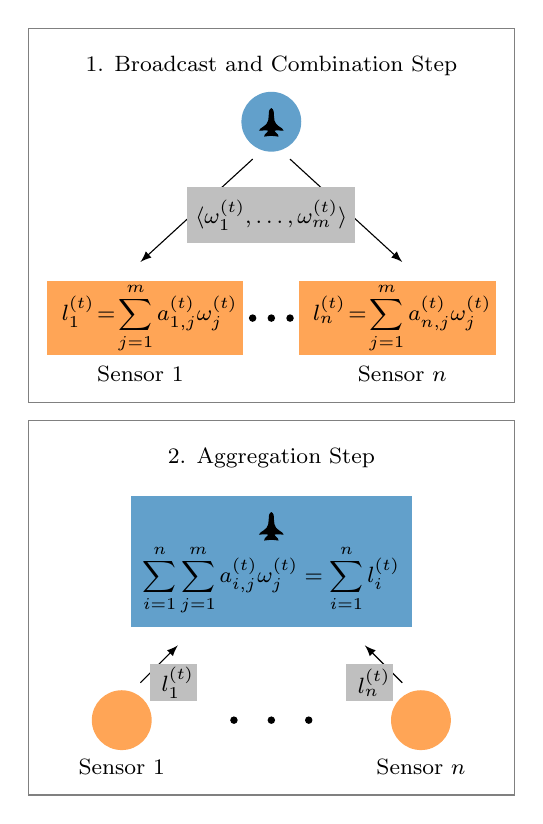
\begin{tikzpicture}[font=\footnotesize,scale=0.95]
    % Step 1
    \node at (3.25,5.5) {1. Broadcast and Combination Step};
    % Navigator
    \fill (3.25,4.75) [pyplotblue!70] ellipse (0.4 and 0.4);
    \pic[xscale=0.22,yscale=0.3] at (3.25,4.9225) {plane};
    % Sensors
    \node at (1.5,1.375) {Sensor $1$};
    \fill [pyplotorange!70] (0.25,1.625) rectangle (2.875,2.625);
    \node at (1.625,2.125) {$\displaystyle l_1^{(t)} \!=\! \sum^m_{j=1}a_{1,j}^{(t)}\omega_j^{(t)}$};
    \node at (5,1.375) {Sensor $n$};
    \fill [pyplotorange!70] (3.625,1.625) rectangle (6.25,2.625);
    \node at (5,2.125) {$\displaystyle l_n^{(t)} \!=\! \sum^m_{j=1}a_{n,j}^{(t)}\omega_j^{(t)}$};
    \fill [black] (3.5,2.125) circle (0.05);
    \fill [black] (3,2.125) circle (0.05);
    \fill [black] (3.25,2.125) circle (0.05);
    % Lines
    \draw [-latex] plot[smooth, tension=.7] coordinates {(3.5,4.25) (5,2.875)};
    \draw [-latex] plot[smooth, tension=.7] coordinates {(3,4.25) (1.5,2.875)};
    \fill [lightgray] (2.125,3.875) rectangle (4.375,3.125);
    \node at (3.25,3.5) {$\langle\omega_1^{(t)},\dots ,\omega_m^{(t)}\rangle$};
    
    % Step 2
    \node at (3.25,0.25) {2. Aggregation Step};
    % Navigator
    \fill [pyplotblue!70] (1.375,-2) rectangle (5.125,-0.25);
    \pic[xscale=0.22,yscale=0.3] at (3.25,-0.4775) {plane};
    \node at (3.25,-1.375) {$\displaystyle \sum^{n}_{i=1}\sum^{m}_{j=1} a_{i,j}^{(t)}\omega_j^{(t)} = \sum^n_{i=1}l^{(t)}_{i}$};
    % Sensors
    \node at (1.25,-3.875) {Sensor $1$};
    \fill  (5.25,-3.25) [pyplotorange!70] ellipse (0.4 and 0.4);
    \node at (5.25,-3.875) {Sensor $n$};
    \fill  (1.25,-3.25) [pyplotorange!70] ellipse (0.4 and 0.4);
    \fill [black] (2.75,-3.25) circle (0.05);
    \fill [black] (3.75,-3.25) circle (0.05);
    \fill [black] (3.25,-3.25) circle (0.05);
    % Lines
    \draw [-latex] plot[smooth, tension=.7] coordinates {(5,-2.75) (4.5,-2.25)};
    \draw [-latex] plot[smooth, tension=.7] coordinates {(1.5,-2.75) (2,-2.25)};
    \fill [lightgray] (1.625,-2.5) rectangle (2.25,-3);
    \node at (2,-2.75) {$l_1^{(t)}$};
    \fill [lightgray] (4.25,-2.5) rectangle (4.875,-3);
    \node at (4.625,-2.75) {$l_n^{(t)}$};
    
    % Bounding rectangles
    \draw [gray] (0,6) rectangle (6.5,1);
    \draw [gray] (0,0.75) rectangle (6.5,-4.25);
\end{tikzpicture}
\caption{Required linear combination aggregation steps at instance $t$.}
\label{fig:agg_steps}
\end{figure}
In addition, we note that an alternative approach to the two-step protocol is computing $\sum^{m}_{j=1}(\omega_j^{(t)}\sum^{n}_{i=1} a_{i,j}^{(t)})$ at the navigator, requiring only values $a_{i,j}^{(t)}, j\in\{1,\dots,m\}$ to be sent from each sensor $i$. We justify the use of bi-directional communication by reducing communication costs when the number of weights is larger than the number of sensors, $m>n$, and by sending fewer weights in the presence of repeats, as will be shown to be the case in section \ref{sec:priv_localisation}.

Before giving a formal definition for the construction and security of our desired encryption scheme, we make the following assumptions on the capabilities of the participants.
\begin{LaTeXdescription}
    \item[Global Navigator Broadcast] We assume that broadcast information from the navigator is received by \textit{all} sensors involved in the protocol.
    \item[Consistent Navigator Broadcast] We assume that broadcast information from the navigator is received equally by all sensors. This means the navigator may not send different weights to individual sensors during a single instance $t$.
    \item[Honest-but-Curious Sensors] We adopt the honest-but-curious attacker model for all involved sensors, meaning that they follow the localisation procedure correctly but may store or use any gained sensitive information.
\end{LaTeXdescription}
We justify the global broadcast assumption by noting that any subset of sensors within the range of the navigator can be considered a complete group and treated as the global set for estimation purposes, generalising the method, while the wide-spread use of cheap non-directional antennas supports the assumption of consistent broadcasts. The final assumption refers to the known problem of misbehaving sensors \cite{lazosSeRLocSecureRangeindependent2004,ben-galOutlierDetection2005}, often requiring additional complicated detection mechanisms, and will not be considered in this work.

We are now ready to define the type of encryption scheme we want for the specified communication protocol and the security guarantees it should provide. We let a linear combination aggregation scheme be defined as a tuple of the four algorithms $(\mathsf{Setup}, \mathsf{Enc}, \mathsf{CombEnc}, \mathsf{AggDec})$. These will be used by a trusted setup party, the navigator and sensors $i\in\{1,\dots,n\}$. They are defined as follows.
\begin{LaTeXdescription}
    \item[$\mathsf{Setup}(\kappa)$] On input of security parameter $\kappa$, generate public parameters $\mathsf{pub}$, the number of weights $m$, the navigator's public and private keys $pk_0$ and $sk_0$ and the sensor private keys $sk_i,\,i\in\{1,\dots,n\}$.
    \item[$\mathsf{Enc}(pk_0, x)$] The navigator and sensors can encrypt any value $x$ with the navigator's public key $pk_0$ and obtain the encryption $\mathcal{E}_{pk_0}(x)$.
    \item[$\mathsf{CombEnc}(t, pk_0, sk_i, \mathcal{E}(\omega_1^{(t)}),\dots,\mathcal{E}(\omega_m^{(t)}), a^{(t)}_{i,1},\dots,a^{(t)}_{i,m})$] At instance $t$, sensor $i$ computes and obtains the encrypted linear combination denoted $l^{(t)}_i = \mathcal{E}_{pk_0,sk_i}(\sum^m_{j=1}a^{(t)}_{i,j}\omega^{(t)}_j)$ using its secret key $sk_i$.
    \item[$\mathsf{AggDec}(t, pk_0, sk_0, l^{(t)}_1,\dots,l^{(t)}_n)$] At instance $t$, the navigator computes the aggregation of linear combinations $\sum^{n}_{i=1}l_i^{(t)}=\sum^{n}_{i=1}\sum^{m}_{j=1} a^{(t)}_{i,j}\omega^{(t)}_j$ using its public and private keys $pk_0$, $sk_0$.
\end{LaTeXdescription}
The security notions we want these algorithms to meet reflect the previously stated estimation privacy goals. The navigator should learn no information from individual sensors while sensors should learn no information from the navigator or any other sensors. In the context of the introduced communication protocol, this can be summarised as the following notions.
\begin{LaTeXdescription}
    \item[Indistinguishable Weights] No colluding subset of sensors gains any new knowledge about the navigator weights $\omega^{(t)}_j,\,j\in\{1,\dots,m\}$ when receiving only their encryptions from the current and previous instances and having the ability to encrypt plaintexts of their choice.
    \item[Linear Combination Aggregator Obliviousness] No colluding subset \textit{excluding} the navigator gains additional information about the remaining sensor values to be weighted, $a^{(t)}_{i,j},\,j\in\{1,\dots,m\}$, where sensor $i$ is not colluding, given only encryptions of their linear combinations $l_i$ from the current and previous instances. Any colluding subset \textit{including} the navigator learns only the sum of all linear combinations weighted by weights of their choice, $\sum^{n}_{i=1}l_i^{(t)}=\sum^{n}_{i=1}\sum^{m}_{j=1} a^{(t)}_{i,j}\omega^{(t)}_j$.
\end{LaTeXdescription}
While indistinguishable weights can be achieved by encrypting weights with an encryption scheme meeting the notion of Indistinguishability under the Chosen Plaintext Attack (IND-CPA) \cite{katzIntroductionModernCryptography2008}, the novel notion of Linear Combination Aggregator Obliviousness (LCAO) has been formalised as a typical cryptographic game between attacker and challenger in appendix \ref{app:lcao}. Lastly, we conclude the cryptographic problem definition with the following important remark.
\begin{remark}
    A leakage function including weights from the navigator requires extra care to be taken when giving its definition. If an attacker compromises the navigator, they have control over the weights, and therefore the leakage function. We note that in the leakage function above, $\sum^n_{i=1}\sum^m_{j=1}a^{(t)}_{i,j}\omega^{(t)}_j$, an individual sum weighted by the same weight may be learned by an attacker, \textit{e.g.}, $\sum^n_{i=1}a^{(t)}_{i,1}$ given weights $(1,0,\dots,0)$, but that individual sensor values $a^{(t)}_{i,j}$ remain private due to the assumption of a consistent broadcast.
\end{remark}

% 
% ########  ######  ########    ########  ########   #######  ########  
% ##       ##    ##    ##       ##     ## ##     ## ##     ## ##     ## 
% ##       ##          ##       ##     ## ##     ## ##     ## ##     ## 
% ######    ######     ##       ########  ########  ##     ## ########  
% ##             ##    ##       ##        ##   ##   ##     ## ##     ## 
% ##       ##    ##    ##       ##        ##    ##  ##     ## ##     ## 
% ########  ######     ##       ##        ##     ##  #######  ########  
% 

\subsection{Estimation problem} \label{subsec:est_problem}
The estimation problem we consider, for which we will reformulate communication to the protocol above, is localisation with range-only sensors. In this work, we will focus on the two-dimensional case for simplicity but will derive methods suitable for extension to a three-dimensional equivalent. The state that we wish to estimate must capture the navigator position, $x$ and $y$, and may contain any other components relevant to the system. It is of the form
\begin{equation}
    \vec{x} = 
    \begin{bmatrix}
        x & y & \cdots
    \end{bmatrix}^\top\,. \label{eqn:state_definition}
\end{equation}
This state evolves following some known system model, which at timestep $k$ can be written as
\begin{equation}
    \vec{x}_k = \vec{f}_k(\vec{x}_{k-1}, \vec{w}_k)\,, \label{eqn:system_model}
\end{equation}
with noise term $\vec{w}_k$. Measurements of $\vec{x}_k$ follow a measurement model dependent on sensor $i\in\{1,\dots,n\}$, given by 
\begin{equation}
    z_{k,i} = h_i(\vec{x}_k)+v_{k,i}\,, \label{eqn:measurement_model}
\end{equation}
with Gaussian measurement noises $v_{k,i} \sim \mathcal{N}(0,r_{k,i})$ and measurement function
\begin{equation}
    \begin{split}
        h_i(\vec{x}) &= \left\lVert
        \begin{bmatrix}
            x & y
        \end{bmatrix}^\top
        - \vec{s}_{i}\right\rVert \\
        &= \sqrt{(x-s_{x,i})^2 + (y-s_{y,i})^2}\,,
    \end{split}
\end{equation}
where
\begin{equation}
    \vec{s}_i = 
    \begin{bmatrix}
        s_{x,i} & s_{y,i}
    \end{bmatrix}^\top
\end{equation} 
is the location of sensor $i$.

We aim to provide a filter that estimates the navigator's state $\vec{x}_k$, at every timestep $k$, without learning sensor positions $\vec{s}_i$, measurements $z_{k,i}$ and measurement variances $r_{k,i}$ beyond the information in the corresponding aggregation leakage function. Similarly, sensors should not learn any information about current state estimates or any other sensor information. Leakage will be further discussed in section \ref{subsec:leakage}, but we note that from any sequential state estimates, following known models, some sensor information leakage can be computed by the navigator. In the context of our leakage function, we will show that this corresponds to the global sums of private sensor information, while individual, or subsets of sensors', information remain private. Similarly, corrupted sensors with access to one or more measurements can produce state estimates of their own, leaking information about navigator state estimates, however, the most accurate estimates, requiring all measurements, will always remain private to the navigator.

% 
% 8888888b.  8888888b.  8888888888 888      8888888 888b     d888  .d8888b.  
% 888   Y88b 888   Y88b 888        888        888   8888b   d8888 d88P  Y88b 
% 888    888 888    888 888        888        888   88888b.d88888 Y88b.      
% 888   d88P 888   d88P 8888888    888        888   888Y88888P888  "Y888b.   
% 8888888P"  8888888P"  888        888        888   888 Y888P 888     "Y88b. 
% 888        888 T88b   888        888        888   888  Y8P  888       "888 
% 888        888  T88b  888        888        888   888   "   888 Y88b  d88P 
% 888        888   T88b 8888888888 88888888 8888888 888       888  "Y8888P"  
%                                                                            
%                                                                            
%                                                                            
% 

\section{Preliminaries} \label{sec:preliminaries}
When proposing an encryption scheme meeting the LCAO notion, we will base our method on the additively homomorphic Paillier encryption scheme \cite{paillierPublicKeyCryptosystemsBased1999} and the Joye-Libert privacy-preserving aggregation scheme \cite{joyeScalableSchemePrivacyPreserving2013}. These schemes have been summarised below. Additionally, the estimation problem we consider uses real-valued inputs and functions and will require encoding real numbers for use with the aforementioned encryption schemes. The method used for encoding has been summarised afterwards.

% 
% ########     ###    #### ##       ##       #### ######## ########  
% ##     ##   ## ##    ##  ##       ##        ##  ##       ##     ## 
% ##     ##  ##   ##   ##  ##       ##        ##  ##       ##     ## 
% ########  ##     ##  ##  ##       ##        ##  ######   ########  
% ##        #########  ##  ##       ##        ##  ##       ##   ##   
% ##        ##     ##  ##  ##       ##        ##  ##       ##    ##  
% ##        ##     ## #### ######## ######## #### ######## ##     ## 
% 

\subsection{Paillier Encryption Scheme} \label{subsec:paillier_scheme}
The Paillier encryption scheme \cite{paillierPublicKeyCryptosystemsBased1999} is an additively homomorphic encryption scheme that bases its security on the decisional composite residuosity assumption (DCRA) and meets the security notion of IND-CPA. Key generation of the Paillier scheme is performed by choosing two sufficiently large primes $p$ and $q$, and computing $N=pq$. A generator $g$ is also required for encryption, which is often set to $g=N+1$ when $p$ and $q$ are of equal bit length \cite{katzIntroductionModernCryptography2008}. The public key is defined by $(N, g)$ and the secret key by $(p, q)$.

Encryption of a plaintext message $a \in \mathbb{Z}_N$, producing ciphertext $c \in \mathbb{Z}^{*}_{N^2}$, is computed by
\begin{equation}
    c = g^a \rho^N \pmod{N^2}
\end{equation}
for a randomly chosen $\rho \in \mathbb{Z}_{N}$. Here, $\rho^N$ can be considered the noise term which hides the value $g^a \pmod{N^2}$, which due to the scheme construction, is an easily computable discrete logarithm. The decryption of a ciphertext is computed by
\begin{equation}
    a = \frac{L(c^\lambda\pmod{N^2})}{L(g^\lambda\pmod{N^2})} \pmod{N}
\end{equation}
where $\lambda = \mathsf{lcm}(p-1, q-1)$ and $L(u) = \frac{u-1}{N}$.

In addition to encryption and decryption, the following homomorphic functions are provided by the Paillier scheme. $\forall a_1,a_2 \in \mathbb{Z}_N$,
\begin{align}
    \mathcal{D}(\mathcal{E}(a_1)\mathcal{E}(a_2) \hspace{-7pt} \pmod{N^2}) &= a_1+a_2 \hspace{-7pt} \pmod{N}\,, \label{eqn:paillier_hom_add}\\
    \mathcal{D}(\mathcal{E}(a_1)g^{a_2} \hspace{-7pt} \pmod{N^2}) &= a_1+a_2\hspace{-7pt}\pmod{N}\,, \label{eqn:paillier_hom_plain_add}\\
    \mathcal{D}(\mathcal{E}(a_1)^{a_2} \hspace{-7pt} \pmod{N^2}) &= a_1a_2 \hspace{-7pt} \pmod{N}\,. \label{eqn:paillier_hom_mult}
\end{align}

% 
%       ##         ##    ## 
%       ##          ##  ##  
%       ##           ####   
%       ## #######    ##    
% ##    ##            ##    
% ##    ##            ##    
%  ######             ##    
% 

\subsection{Joye-Libert Privacy-Preserving Aggregation Scheme} \label{subsec:joye_libert_scheme}
The Joye-Libert privacy-preserving aggregation scheme \cite{joyeScalableSchemePrivacyPreserving2013} is a scheme defined on time-series data and meets the security notion of Aggregator Obliviousness (AO) \cite{shiPrivacyPreservingAggregationTimeSeries2011}. Similarly to the Paillier scheme, it bases its security on the DCRA. A notable difference to a public-key encryption scheme is its need for a trusted party to perform the initial key generation and distribution.

Key generation is computed by first choosing two equal-length and sufficiently large primes $p$ and $q$, and computing $N=pq$. A hash function $H:\mathbb{Z} \rightarrow \mathbb{Z}_{N^2}^*$ is defined and the public key is set to $(N, H)$. $n$ private keys are generated by choosing $sk_i,\,i\in\{1,\dots,n\}$, uniformly from $\mathbb{Z}_{N^2}$ and distributing them to $n$ participants (whose values are to be aggregated), while the last key is set as
\begin{equation}
    sk_0 = -\sum^{n}_{i=1}sk_i \pmod{N^2}\,,
\end{equation}
and sent to the aggregator.

Encryption of plaintext $a^{(t)}_{i} \in \mathbb{Z}_N$ to ciphertext $c^{(t)}_{i} \in \mathbb{Z}_{N^2}$ at instance $t$ is computed by user $i$ as
\begin{equation}
    c^{(t)}_{i} = (N+1)^{a^{(t)}_{i}} H(t)^{sk_i} \pmod{N^2}\,.
\end{equation}
Here, we can consider $H(t)^{sk_i}$ the noise term which hides the easily computable discrete logarithm $g^{a^{(t)}_{i}} \pmod{N^2}$, where $g=N+1$ (as with the Paillier scheme above).

When all encryptions $c^{(t)}_{i},\,i\in\{1,\dots,n\}$ are sent to the aggregator, summation and decryption of the aggregated sum are computed by the functions
\begin{equation}
    c^{(t)} = H(t)^{sk_0}\prod^{n}_{i=1}c^{(t)}_{i} \pmod{N^2} \label{eqn:agg_summation}
\end{equation}
and
\begin{equation}
    \sum^{n}_{i=1}a^{(t)}_{i} = \frac{c^{(t)}-1}{N} \pmod{N}\,. \label{eqn:agg_decryption}
\end{equation}
Correctness follows from $\sum^{n}_{i=0}sk_i = 0$, and thus
\begin{equation*}
    \begin{split}
        &H(t)^{sk_0}\prod^{n}_{i=1}c_{i,t} \pmod{N^2} \\
        \equiv &H(t)^{sk_0}\prod^{n}_{i=1}(N+1)^{a_{i,t}} H(t)^{sk_i} \pmod{N^2} \\
        \equiv &H(t)^{\sum^n_{j=0}sk_j} \prod^{n}_{i=1}(N+1)^{a_{i,t}} \pmod{N^2} \\
        \equiv &(N+1)^{\sum^n_{i=1}a_{i,t}} \pmod{N^2}\,,
    \end{split}
\end{equation*}
removing all noise terms.

% 
% ######## ##    ##  ######   #######  ########  #### ##    ##  ######   
% ##       ###   ## ##    ## ##     ## ##     ##  ##  ###   ## ##    ##  
% ##       ####  ## ##       ##     ## ##     ##  ##  ####  ## ##        
% ######   ## ## ## ##       ##     ## ##     ##  ##  ## ## ## ##   #### 
% ##       ##  #### ##       ##     ## ##     ##  ##  ##  #### ##    ##  
% ##       ##   ### ##    ## ##     ## ##     ##  ##  ##   ### ##    ##  
% ######## ##    ##  ######   #######  ########  #### ##    ##  ######   
% 

\subsection{Integer Encoding for Real Numbers} \label{subsec:encoding}
In both the Paillier and Joye-Libert schemes, as well as the one we introduce, meaningful inputs $a$ are bounded to $a \in \mathbb{Z}_N$. For this reason, real-valued estimation variables require quantisation and integer mapping for encryption and aggregation. We will rely on a generalised Q number encoding \cite{oberstarFixedPointRepresentationFractional2007} due to implementation simplicity and applicability.

We will consider a subset of rational numbers in terms of a range $M \in \mathbb{N}$ and fractional precision $\phi \in \mathbb{N}$. This contrasts with the common definition in terms of total and fractional bits \cite{oberstarFixedPointRepresentationFractional2007,schulzedarupEncryptedCooperativeControl2019,farokhiSecurePrivateControl2017}, but allows for a direct mapping to integer ranges which are not a power of two. A rational subset $\mathbb{Q}_{M,\phi}$ is then given by
\begin{equation}
    \mathbb{Q}_{M,\phi} = \left\{q \,\middle|\, \phi q \in \mathbb{N} \wedge -\left\lfloor\frac{M}{2}\right\rfloor \leq \phi q < \left\lfloor\frac{M}{2}\right\rfloor \right\}\,,
\end{equation}
and we can quantize any real number $a$ by taking the nearest rational $q \in \mathbb{Q}_{M,\phi}$, that is, $\argmin_{q\in\mathbb{Q}_{M,\phi}} |a-q|$. In this form, mapping rationals $\mathbb{Q}_{M,\phi}$ to an encryption range $\mathbb{Z}_N$ is achieved by choosing $M=N$ and handling negatives by modulo arithmetic. Additionally, we note that the Q number format requires a precision factor $\phi$ to be removed after each encoded multiplication. This is captured by a third parameter $d$; the number of precision factors present in encodings.

The function for \textit{combined} quantisation and encoding, $\mathsf{E}_{M,\phi,d}(a)$, of a given number $a \in \mathbb{R}$ and with an integer range $\mathbb{Z}_M$, precision $\phi$ and scaling for $d$ prior encoded multiplications is given by
\begin{equation}
    \mathsf{E}_{M,\phi,d}(a) = \left\lfloor \phi^{d+1} a \right\rceil \pmod{M}\,. \label{eqn:encode}
\end{equation}
Decoding of an integer $u \in \mathbb{Z}_M$, is given by
\begin{equation}
    \mathsf{E}^{-1}_{M,\phi,d}(u) \!=\! 
    \begin{dcases}
        \frac{u\hspace{-8pt}\pmod{M}}{\phi^{d+1}}, &\hspace{-6pt}u\hspace{-8pt}\pmod{M} \leq \left\lfloor\frac{M}{2}\right\rfloor \\
        -\frac{M - u\hspace{-8pt}\pmod{M}}{\phi^{d+1}}, &\hspace{-6pt}\text{otherwise} \\
    \end{dcases}\!\!.\label{eqn:decode}
\end{equation}

This encoding scheme provides the following homomorphic operations,
\begin{equation}
    \begin{split}
        \mathsf{E}_{M,\phi,d}(a_1) + \mathsf{E}_{M,\phi,d}(a_2)& \pmod{M} =\\
        &\mathsf{E}_{M,\phi,d}(a_1+a_2)
    \end{split}\label{eqn:encoding_homomorphic_add}
\end{equation}
and
\begin{equation}
    \begin{split}
        \mathsf{E}_{M,\phi,d}(a_1)\mathsf{E}_{M,\phi,d}(a_2)& \pmod{M} =\\
        &\mathsf{E}_{M,\phi,d+1}(a_1a_2)\,,
    \end{split}
\end{equation}
noting that when $M=N$, the operations and modulus correspond with those in the Paillier homomorphic operations \eqref{eqn:paillier_hom_add}, \eqref{eqn:paillier_hom_plain_add} and \eqref{eqn:paillier_hom_mult}, and the Joye-Libert sum \eqref{eqn:agg_decryption}.

In general, the choice of a large precision parameter $\phi$ may reduce quantisation errors introduced in \eqref{eqn:encode}, but risks overflow after too many multiplications. Given the largest number of encoded multiplications, $d_{max}$, and the largest value to be encoded $a_{max}$, the parameter should be chosen such that
\begin{equation}
    \left|\phi^{d_{max}+1}a_{max}\right| < \left\lfloor \frac{M}{2} \right\rfloor\,.
\end{equation}
In practice, $N$ is typically very large ($N>2^{1024}$) and this condition can be ignored when $M=N$.

% 
% 888      .d8888b.        d8888  .d88888b.  
% 888     d88P  Y88b      d88888 d88P" "Y88b 
% 888     888    888     d88P888 888     888 
% 888     888           d88P 888 888     888 
% 888     888          d88P  888 888     888 
% 888     888    888  d88P   888 888     888 
% 888     Y88b  d88P d8888888888 Y88b. .d88P 
% 88888888 "Y8888P" d88P     888  "Y88888P"  
%                                            
%                                            
%                                            
% 

\section{Private Linear Combination Aggregation Scheme} \label{sec:lcao_scheme}
In this section, we introduce an encryption scheme meeting the desired security properties in section \ref{subsec:crypto_problem}. The scheme is a combination of the Paillier and Joye-Libert schemes and provides encrypted weights meeting IND-CPA and encrypted aggregation meeting the notion of LCAO defined in section \ref{subsec:crypto_problem}. Similarly to its constituents, the scheme bases its security on the DCRA and, as with the Joye-Libert scheme, requires a trusted party for initial key generation and distribution. 

As aggregation is typically performed on scalar inputs, we extend our notation to the context of multidimensional estimation data by letting an instance $t_{k,\tau}$ uniquely capture the scalar aggregation during an estimation timestep $k$ for a single element with position index $\tau$. To achieve this in practice, any injective function can be used, such as the concatenation $t_{k,\tau}=k\mathbin\|\tau$. The four algorithms defining our scheme are given as follows.
\begin{LaTeXdescription}
    \item[$\mathsf{Setup}(\kappa)$] On input parameter $\kappa$, generate two equal length, sufficiently large, primes $p$ and $q$, and compute $N=pq$. Define a hash function $H:\mathbb{Z} \rightarrow \mathbb{Z}_{N^2}^*$, choose the number of weights to combine, $m>1$, and set public parameter $\mathsf{pub}=H$, navigator public key $pk_0 = N$ and navigator private key $sk_0=(p,q)$. Sensor secret keys are generated by choosing $sk_i,\,i\in\{1,\dots,n-1\}$ uniformly from $\mathbb{Z}_{N^2}$ and setting the last key as $sk_n = -\sum^{n-1}_{i=1}sk_i \pmod{N^2}$.
 
    \item[$\mathsf{Enc}(pk_0, x)$] Public-key encryption is computed by the Paillier encryption scheme with implicit generator $g=N+1$. This is given by
    \begin{equation}
        \mathcal{E}_{pk_0}(x) = (N+1)^{x}\rho^N \pmod{N^2}\,, \label{eqn:our_scheme_encrypt}
    \end{equation}
    for a randomly chosen $\rho \in \mathbb{Z}_N$.

    \item[$\mathsf{CombEnc}(t_{k,\tau}, pk_0, sk_i, \mathcal{E}(\omega_1^{(k,\tau)})\dots , a^{(k,\tau)}_{i,1}\dots )$] At instance $t_{k,\tau}$, encrypted linear combination is computed as 
    \begin{equation}
        l^{(k,\tau)}_i = H(t_{k,\tau})^{sk_i}\prod^{m}_{j=1}\mathcal{E}_{pk_0}(\omega^{(k,\tau)}_j)^{a^{(k,\tau)}_{i,j}} \pmod{N^2}\,,\label{eqn:our_scheme_lin_comb}
    \end{equation}
    and makes use of the homomorphic property \eqref{eqn:paillier_hom_mult}. Correctness follows from
    \begin{equation*}
        \begin{split}
            l^{(k,\tau)}_i &= H(t_{k,\tau})^{sk_i}\prod^{m}_{j=1}\mathcal{E}_{pk_0}(\omega^{(k,\tau)}_j)^{a^{(k,\tau)}_{i,j}} \pmod{N^2} \\
            &= H(t_{k,\tau})^{sk_i}\prod^{m}_{j=1}\mathcal{E}_{pk_0}(a^{(k,\tau)}_{i,j}\omega^{(k,\tau)}_j) \pmod{N^2} \\
            &= H(t_{k,\tau})^{sk_i}\cdot \\
            &\qquad \prod^{m}_{j=1}(N+1)^{a^{(k,\tau)}_{i,j}\omega^{(k,\tau)}_j} \rho^{N}_{j} \pmod{N^2} \\
            &= H(t_{k,\tau})^{sk_i}\cdot \\
            &\qquad (N+1)^{\sum^{m}_{j=1}a^{(k,\tau)}_{i,j}\omega^{(k,\tau)}_j} \rho_{i}^{N} \pmod{N^2}\,,
        \end{split}
    \end{equation*}
    for some values $\rho_i,\rho_j \in \mathbb{Z}_N,\,j\in\{1,\dots,m\}$. Here, $\rho_i^N$ and $H(t_{k,\tau})^{sk_i}$ can be considered the noise terms corresponding to the two levels of encryption from $pk_0$ and $sk_i$, respectively.

    \item[$\mathsf{AggDec}(t_{k,\tau}, pk_0, sk_0, l^{(k,\tau)}_1,\dots,l^{(k,\tau)}_n)$] Aggregation is computed as $l^{(k,\tau)} = \prod^n_{i=1}l^{(k,\tau)}_i \pmod{N^2}$, removing the aggregation noise terms, and is followed by Paillier scheme decryption
    \begin{equation}
        \begin{split}
            \sum^{n}_{i=1}\sum^{m}_{j=1}&a^{(k,\tau)}_{i,j}\omega^{(k,\tau)}_j =\\
            &\frac{L((l^{(k,\tau)})^\lambda\pmod{N^2})}{L((N+1)^\lambda\pmod{N^2})} \pmod{N}\,,
        \end{split} \label{eqn:our_scheme_decrypt}
    \end{equation}
    with $\lambda = \mathsf{lcm}(p-1, q-1)$ and $L(u) = \frac{u-1}{N}$. The correctness of the aggregation can be seen from
    \begin{align*}
        \begin{split}
        l^{(k,\tau)} &= \prod^n_{i=1}H(t_{k,\tau})^{sk_i}\cdot \\
        &\qquad (N+1)^{\sum^{m}_{j=1}a^{(k,\tau)}_{i,j}\omega^{(k,\tau)}_j}\rho_i^N \!\!\pmod{N^2}
        \end{split}\\
        \begin{split}
            &= H(t_{k,\tau})^{\sum^n_{i=1}sk_i}\cdot \\
            &\qquad \prod^n_{i=1}(N+1)^{\sum^{m}_{j=1}a^{(k,\tau)}_{i,j}\omega^{(k,\tau)}_j}\rho_i^N \!\!\pmod{N^2}
        \end{split}\\
        &= (N+1)^{\sum^n_{i=1}\sum^{m}_{j=1}a^{(k,\tau)}_{i,j}\omega^{(k,\tau)}_j}\rho'^N \!\!\pmod{N^2}\,,
    \end{align*}
    for some values $\rho_i,\rho' \in \mathbb{Z}_N,\,i\in\{1,\dots,n\}$.
\end{LaTeXdescription}
Additionally, we note that in the above construction, all weights $\omega^{(k,\tau)}_j$ and values $a^{(k,\tau)}_{i,j}$ are integers and the resulting linear combinations and aggregation are computed modulo $N$. 

The security proof of this scheme must both show that encrypted weights meet IND-CPA and that encrypted aggregation meets LCAO. As weights are encrypted with the Paillier encryption scheme, the first requirement is already met. To show that aggregation meets LCAO, a reduction proof is given in appendix \ref{app:proof}.

\begin{remark}
    Given the construction of the scheme above, it can be seen that any weights $\omega^{(k,\tau)}_j$, whose values are known at each sensor, do not need to be broadcast by the navigator. In this case, sensors can replace
    \begin{equation}
        \mathcal{E}_{pk_0}(\omega^{(k,\tau)}_j)^{a^{(k,\tau)}_{i,j}} = (N+1)^{\omega^{(k,\tau)}_ja^{(k,\tau)}_{i,j}}\rho_j^N \pmod{N^2}
    \end{equation}
    in \eqref{eqn:our_scheme_lin_comb}, by
    \begin{equation}
        (N+1)^{\omega^{(k,\tau)}_ja^{(k,\tau)}_{i,j}} \pmod{N^2}\,.
    \end{equation}
    This is due to the removal of $\rho_j^N$ terms during decryption and can be used to reduce the navigator's broadcast communication cost by the number of weights $\omega^{(k,\tau)}_j$ that do not hold any information private to the navigator and are known by the sensors in advance.
\end{remark}

% 
% 8888888b.  8888888b.  8888888 888     888      888      .d88888b.   .d8888b.  
% 888   Y88b 888   Y88b   888   888     888      888     d88P" "Y88b d88P  Y88b 
% 888    888 888    888   888   888     888      888     888     888 888    888 
% 888   d88P 888   d88P   888   Y88b   d88P      888     888     888 888        
% 8888888P"  8888888P"    888    Y88b d88P       888     888     888 888        
% 888        888 T88b     888     Y88o88P        888     888     888 888    888 
% 888        888  T88b    888      Y888P         888     Y88b. .d88P Y88b  d88P 
% 888        888   T88b 8888888     Y8P          88888888 "Y88888P"   "Y8888P"  
%                                                                               
%                                                                               
%                                                                               
% 

\section{Privacy-Preserving Localisation} \label{sec:priv_localisation}
With a concrete scheme meeting the LCAO notion, we can now put forward a localisation filter with communication that can be reformulated to the required protocol. To produce an estimate of the state $\vec{x}_k$, we make use of an algebraic reformulation of the Extended Kalman Filter (EKF), the Extended Information Filter (EIF) \cite{maybeckStochasticModelsEstimation1982}, which reduces the filter update step to a single summation. The EIF update step requires the predicted state estimate $\hat{\vec{x}}_{k|k-1}$ and estimate covariance $\mat{P}_{k|k-1}$ in the information vector and matrix forms
\begin{equation}
    \hat{\vec{y}}_{k|k-1} = \mat{P}_{k|k-1}^{-1}\hat{\vec{x}}_{k|k-1} \quad\textrm{and}\quad \mat{Y}_{k|k-1} = \mat{P}_{k|k-1}^{-1}\,,
\end{equation}
respectively. In this form, the update equations for $n$ sensor measurements at time $k$, with measurement models \eqref{eqn:measurement_model}, are given by
\begin{equation}
    \begin{split}
        &\hat{\vec{y}}_{k|k} = \hat{\vec{y}}_{k|k-1} + \\
        &\quad \sum^n_{i=1}\mat{H}^\top_{k,i} r^{-1}_i (z_{k,i} - h_i(\hat{\vec{x}}_{k|k-1}) + \mat{H}_{k,i}\hat{\vec{x}}_{k|k-1})
    \end{split} \label{eqn:eif_info_vec_update}
\end{equation}
and
\begin{equation}
    \mat{Y}_{k|k} = \mat{Y}_{k|k-1} + \sum^n_{i=1}\mat{H}^\top_{k,i} r^{-1}_i \mat{H}_{k,i}\,, \label{eqn:eif_info_mat_update}
\end{equation}
with Jacobians
\begin{equation}
    \mat{H}_{k,i} = \left.\frac{\partial h_i}{\partial \vec{x}}\right|_{\hat{\vec{x}}_{k|k-1}} \label{eqn:measurement_jacobian}
\end{equation}
for sensors $i\in\{1,\dots,n\}$. After converting the updated information vector and matrix back to state estimate $\hat{\vec{x}}_{k|k}$ and estimate covariance $\mat{P}_{k|k}$, the filter's prediction step can be computed by the navigator locally using any suitable filter for the known system model \eqref{eqn:system_model}.

In the form above, at every timestep $k$, all sensitive sensor information required for state estimation is captured in the measurement vector
\begin{equation}
    \vec{i}_{k,i} = \mat{H}^\top_{k,i} r^{-1}_i (z_{k,i} - h_i(\hat{\vec{x}}_{k|k-1}) + \mat{H}_{k,i}\hat{\vec{x}}_{k|k-1}) \label{eqn:measurement_vec}
\end{equation}
and the measurement matrix
\begin{equation}
    \mat{I}_{k,i} = \mat{H}^\top_{k,i} r^{-1}_i \mat{H}_{k,i}\,, \label{eqn:measurement_mat}
\end{equation}
namely, their measurements $z_{k,i}$, measurement variances $r_{k,i}$ and locations $\vec{s}_i$; captured in measurement functions $h_i$ and Jacobians $\mat{H}_{k,i}$. However, $\vec{i}_{k,i}$ and $\mat{I}_{k,i}$ also require the current predicted state estimate $\hat{\vec{x}}_{k|k-1}$ to be computed (in $h_i$ and $\mat{H}_{k,i}$). For this reason, our goal is to reformulate \eqref{eqn:measurement_vec} and \eqref{eqn:measurement_mat} to be computable at each sensor $i$ as a linear combination of functions of the navigator state estimate (the navigator weights), to be subsequently aggregated at the navigator. Application of the linear combination aggregation scheme proposed would in turn guarantee that sensors do not learn the navigator state, and the navigator learns only the aggregation required for updating its state estimate in \eqref{eqn:eif_info_vec_update} and \eqref{eqn:eif_info_mat_update}.

% 
% ########     ###    ##    ##  ######   ########    ##     ##  #######  ########  
% ##     ##   ## ##   ###   ## ##    ##  ##          ###   ### ##     ## ##     ## 
% ##     ##  ##   ##  ####  ## ##        ##          #### #### ##     ## ##     ## 
% ########  ##     ## ## ## ## ##   #### ######      ## ### ## ##     ## ##     ## 
% ##   ##   ######### ##  #### ##    ##  ##          ##     ## ##     ## ##     ## 
% ##    ##  ##     ## ##   ### ##    ##  ##          ##     ## ##     ## ##     ## 
% ##     ## ##     ## ##    ##  ######   ########    ##     ##  #######  ########  
% 

\subsection{Range Measurement Modification} \label{subsec:range_measurement_mod}

The first thing we notice when wanting to decompose $\vec{i}_{k,i}$ and $\mat{I}_{k,i}$ to a linear combination of functions of $\hat{\vec{x}}_{k|k-1}$, is that $h_i$ cannot be rearranged in this way due to the present square-root. Similarly, the Jacobian of $h_i$ at $\hat{\vec{x}}_{k|k-1}$,
\begin{equation}
    \mat{H}_{k,i} = 
    \begin{bmatrix}
        \frac{\hat{x}_{k|k-1} - s_{x,i}}{\sqrt{(\hat{x}_{k|k-1} - s_{x,i})^2 + (\hat{y}_{k|k-1} - s_{y,i})^2}} \\
        \frac{\hat{y}_{k|k-1} - s_{y,i}}{\sqrt{(\hat{x}_{k|k-1} - s_{x,i})^2 + (\hat{y}_{k|k-1} - s_{y,i})^2}} \\
        0 \\
        \vdots
    \end{bmatrix}\,,
\end{equation}
cannot be either. We, therefore, consider the modified measurement functions
\begin{equation}
    h'_i(\vec{x}) = h_i(\vec{x})^2\,. \label{eqn:modified_measurement_func}
\end{equation}
A measurement function in this form allows rearrangement of $h'_i$ and the corresponding Jacobian $\mat{H}'_{k,i}$ to a linear combination of powers of location elements in $\hat{\vec{x}}_{k|k-1}$, as
\begin{equation}
    \begin{split}
        h'_i(\vec{x}) &= \left\lVert
        \begin{bmatrix}
            x & y
        \end{bmatrix}^\top - \vec{s}_i\right\rVert^2 \\
        &= (x - s_{x,i})^2 + (y - s_{y,i})^2 \\
        &= x^2 + y^2 -2s_{x,i}x -2s_{y,i}y +s_{x,i}^2 +s_{y,i}^2
    \end{split}\,,
\end{equation}
and
\begin{equation}
    \mat{H}'_{k,i} = 
    \begin{bmatrix}
        2\hat{x}_{k|k-1} - 2s_{x,i} \\
        2\hat{y}_{k|k-1} - 2s_{y,i} \\
        0 \\
        \vdots
    \end{bmatrix}\,. \label{eqn:modified_jacobian}
\end{equation}
Here, $h'_i$ and $\mat{H}'_{k,i}$ are linear combinations of $\hat{x}_{k|k-1}^2$, $\hat{y}_{k|k-1}^2$, $\hat{x}_{k|k-1}$ and $\hat{y}_{k|k-1}$. To show how the corresponding modified measurement vectors $\vec{i}'_{k,i}$ and matrices $\mat{I}'_{k,i}$ can be similarly rearranged and used for localisation, we also require the existence of measurements following a modified measurement model of the form
\begin{equation}
    z'_{k,i} = h'_i(\vec{x}_k)+v'_{k,i}\,, \label{eqn:modified_measurement_model}
\end{equation}
where $z'_{k,i}$ is the modified measurement, and noise term $v'_{k,i}$ is zero-mean and has a known variance $r'_{k,i}$.

Computing $z'_{k,i}$ and its variance $r'_{k,i}$ from the original measurements $z_{k,i}$ are complicated by the noise term $v_{k,i} \sim \mathcal{N}(0, r_{k,i})$, and simply squaring the original range measurements produces
\begin{equation}
    \begin{split}
        z_{k,i}^2 &= (h_i(\vec{x}_k) + v_{k,i})^2 \\
        &= h'_i(\vec{x}_k) + 2h_i(\vec{x}_k)v_{k,i} + v_{k,i}^2\,,
    \end{split}
\end{equation}
with a new noise term $2h_i(\vec{x}_k)v_{k,i} + v_{k,i}^2$, now dependent on the measurement function $h_i$, and no longer zero-mean. We can compute the mean of this new noise term (a function of the Gaussian term $v_{k,i}$) as $\mathsf{E}[2h_i(\vec{x}_k)v_{k,i} + v_{k,i}^2] = r_{k,i}$ and mean-adjust modified measurements as
\begin{equation}
    \begin{split}
        z'_{k,i} &= z_{k,i}^2 - r_{k,i} \\
        &= h_i(\vec{x}_k)^2 + 2h_i(\vec{x}_k)v_{k,i} + v_{k,i}^2 - r_{k,i} \\
        &= h'_i(\vec{x}_k) + v'_{k,i}\,,
    \end{split} \label{eqn:modified_measurement}
\end{equation}
with now zero-mean noise $v'_{k,i} = 2h_i(\vec{x}_k)v_{k,i} + v_{k,i}^2 - r_{k,i}$. The noise in this case (again a function of $v_{k,i}$) has variance 
\begin{equation}
    \mathsf{Var}[v'_{k,i}] = 4h_i(\vec{x}_k)^2r_{k,i} + 2r_{k,i}^2 \label{eqn:modified_measurement_variance}
\end{equation}
and is also dependent on $h_i$. To use the modified measurement \eqref{eqn:modified_measurement} with the EIF, we require an estimate for $\mathsf{Var}[v'_{k,i}]$ at the sensor as well. Additionally, a conservative estimate (\textit{i.e.}, a larger variance resulting in less confidence in measurements) is desirable to reduce filter divergence. While the naive approach, replacing $h_i(\vec{x}_k)$ with $z_{k,i}$ in \eqref{eqn:modified_measurement_variance}, may not provide a conservative estimate when $z_{k,i}^2 < h_i(\vec{x}_k)^2$, the Gaussianity of $v_{k,i}$ can be exploited to provide a conservative estimate with $95\%$ confidence by shifting the replacement term $z_{k,i}$ by two of its standard deviations $\sqrt{r_{k,i}}$. The modified measurement's variance at timestep $k$ can therefore be conservatively approximated by
\begin{equation}
    \begin{split}
        r'_{k, i} &= 4(z_{k,i} + 2\sqrt{r_{k,i}})^2r_{k,i} + 2r_{k,i}^2 \\
        &\gtrapprox \mathsf{Var}[v'_{k,i}]\,,
    \end{split} \label{eqn:modified_measurement_variance_estimate}
\end{equation}
at each sensor $i$.

The modified measurement model \eqref{eqn:modified_measurement_model} can now be used for localisation, when measurements are modified by \eqref{eqn:modified_measurement} and their new variance estimated with \eqref{eqn:modified_measurement_variance_estimate}.

% 
% ##        #######   ######  
% ##       ##     ## ##    ## 
% ##       ##     ## ##       
% ##       ##     ## ##       
% ##       ##     ## ##       
% ##       ##     ## ##    ## 
% ########  #######   ######  
% 

\subsection{Localisation} \label{subsec:localisation}
To complete the EIF update as a linear combination aggregation, modified vectors $\vec{i}'_{k,i}$ and matrices $\mat{I}'_{k,i}$, using the modified measurement model \eqref{eqn:modified_measurement_model}, can be rearragned as follows.
\begin{equation}
    \begin{split}
        \vec{i}'_{k,i} &= \mat{H}_{k,i}^{\prime\top} r_{k,i}^{\prime-1}(z'_{k,i} - h'_i(\hat{\vec{x}}_{k|k-1}) + \mat{H}'_{k,i}\hat{\vec{x}}_{k|k-1}) \\
        &= 
        \begin{bmatrix}
            \alpha_i^{(k,1)} & \alpha_i^{(k,2)} & 0 & \cdots
        \end{bmatrix}^\top\,,
    \end{split} \label{eqn:hrz_linear_comb}
\end{equation}
with
\begin{align*}
    \begin{split}
        \alpha_i^{(k,1)} &= (2r_{k,i}^{\prime-1})\hat{x}_{k|k-1}^3 + (2r_{k,i}^{\prime-1})\hat{x}_{k|k-1}\hat{y}_{k|k-1}^2 \\
        &\quad+ (-r_{k,i}^{\prime-1}s_{x,i})\hat{x}_{k|k-1}^2 + (-2r_{k,i}^{\prime-1}s_{x,i})\hat{y}_{k|k-1}^2 \\
        &\quad+ (2r_{k,i}^{\prime-1}z'_{k,i})\hat{x}_{k|k-1} + (-2r_{k,i}^{\prime-1}s_{x,i}^2)\hat{x}_{k|k-1}\\
        &\quad+ (-2r_{k,i}^{\prime-1}s_{y,i}^2)\hat{x}_{k|k-1} + (2r_{k,i}^{\prime-1}s_{x,i}^3) \\
        &\quad+ (2r_{k,i}^{\prime-1}s_{x,i}s_{y,i}^2) + (-2r_{k,i}^{\prime-1}s_{x,i} z'_{k,i})\ \textrm{and}
    \end{split}\\
    \begin{split}
        \alpha_i^{(k,2)} &= (2r_{k,i}^{\prime-1})\hat{y}_{k|k-1}^3 + (2r_{k,i}^{\prime-1})\hat{x}_{k|k-1}^2\hat{y}_{k|k-1} \\
        &\quad+ (-2r_{k,i}^{\prime-1}s_{y,i})\hat{x}_{k|k-1}^2 + (-2r_{k,i}^{\prime-1}s_{y,i})\hat{y}_{k|k-1}^2 \\
        &\quad+ (2r_{k,i}^{\prime-1}z'_{k,i})\hat{y}_{k|k-1} + (-2r_{k,i}^{\prime-1}s_{x,i}^2)\hat{y}_{k|k-1} \\
        &\quad+ (-2r_{k,i}^{\prime-1}s_{y,i}^2)\hat{y}_{k|k-1} + (2r_{k,i}^{\prime-1}s_{y,i}s_{x,i}^2) \\
        &\quad+ (2r_{k,i}^{\prime-1}s_{y,i}^3) + (-2r_{k,i}^{\prime-1}s_{y,i}z'_{k,i})\,,
    \end{split}
\end{align*}
and
\begin{equation}
    \begin{split}
        \mat{I}'_{k,i} &= \mat{H}_{k,i}^{\prime\top} r_{k,i}^{\prime-1}\mat{H}'_{k,i} \\
        &=
        \begin{bmatrix}
            \alpha_i^{(k,3)} & \alpha_i^{(k,4)} & 0 & \cdots \\
            \alpha_i^{(k,5)} & \alpha_i^{(k,6)} & 0 & \cdots\\
            0 & 0 & 0 & \cdots \\
            \vdots & \vdots & \vdots & \ddots
        \end{bmatrix}\,,
    \end{split} \label{eqn:hrh_linear_comb}
\end{equation}
with
\begin{align*}
    \begin{split}
        \alpha_i^{(k,3)} &= (4r_{k,i}^{\prime-1})\hat{x}_{k|k-1}^2 + (-8r_{k,i}^{\prime-1}s_{x,i})\hat{x}_{k|k-1} \\
        &\qquad+ (4r_{k,i}^{\prime-1}s_{x,i}^2)\,,
    \end{split}\\
    \begin{split}
        \alpha_i^{(k,4)} &= (4r_{k,i}^{\prime-1})\hat{x}_{k|k-1}\hat{y}_{k|k-1} + (-4r_{k,i}^{\prime-1}s_{y,i})\hat{x}_{k|k-1}  \\
        &\qquad+ (-4r_{k,i}^{\prime-1}s_{x,i})\hat{y}_{k|k-1} + (4r_{k,i}^{\prime-1}s_{x,i}s_{y,i})\,,
    \end{split}\\
    \alpha_i^{(k,5)} &= \alpha_i^{(k,4)}\ \textrm{and} \\
    \begin{split}
        \alpha_i^{(k,6)} &= (4r_{k,i}^{\prime-1})\hat{y}_{k|k-1}^2 + (-8r_{k,i}^{\prime-1}s_{y,i})\hat{y}_{k|k-1} \\
        &\qquad+ (4r_{k,i}^{\prime-1}s_{y,i}^2)\,.
    \end{split}
\end{align*}
The above rearrangements give $\vec{i}'_{k,i}$ and $\mat{I}'_{k,i}$ as linear comabinations of elements in
\begin{equation}
    \begin{split}
        &\{ \hat{x}_{k|k-1}^3,\ \hat{y}_{k|k-1}^3,\ \hat{x}_{k|k-1}^2\hat{y}_{k|k-1},\ \hat{x}_{k|k-1}\hat{y}_{k|k-1}^2,\\
        &\quad \hat{x}_{k|k-1}^2,\ \hat{y}_{k|k-1}^2,\ \hat{x}_{k|k-1}\hat{y}_{k|k-1},\ \hat{x}_{k|k-1},\ \hat{y}_{k|k-1}\}\,,
    \end{split} \label{eqn:weights_to_broadcast}
\end{equation}
which capture all of the private state information in $\hat{\vec{x}}_{k|k-1}$ required at the sensors. The corresponding EIF update steps \eqref{eqn:eif_info_vec_update} and \eqref{eqn:eif_info_mat_update} then become
\begin{equation}
    \hat{\vec{y}}_{k|k} = \hat{\vec{y}}_{k|k-1} + \sum^n_{i=1}\vec{i}'_{k,i} \label{eqn:eif_modified_vec_update}
\end{equation}
and
\begin{equation}
    \mat{Y}_{k|k} = \mat{Y}_{k|k-1} + \sum^n_{i=1}\mat{I}'_{k,i}\,, \label{eqn:eif_modified_mat_update}
\end{equation}
respectively.
\begin{remark}
    The above has been derived for two-dimensional localisation but can be similarly derived for the three-dimensional case. However, the number of weights increases combinatorially with the number of dimensions, thus affecting the cost of communication as well.
\end{remark}

% 
%    ###    ##        ######   
%   ## ##   ##       ##    ##  
%  ##   ##  ##       ##        
% ##     ## ##       ##   #### 
% ######### ##       ##    ##  
% ##     ## ##       ##    ##  
% ##     ## ########  ######   
% 

\subsection{Pseudocode} \label{subsec:pseudocode}
Measurement modification, real number encoding and linear combination aggregation are all required to compute the modified EIF from the previous section in a privacy-preserving manner. In this section, we summarise this entire localisation process and give the pseudocode for its execution. For brevity, we will assume $\phi$ and $M=N$ from section \ref{subsec:encoding} to be public information and thus simplify the encoding notation $\mathsf{E}_{N,\phi,d}(\cdot)$ to $\mathsf{E}_{d}(\cdot)$. The privacy-preserving localisation filter consists of the following steps.
\begin{LaTeXdescription}
    \item[Setup] The $\mathsf{Setup}$ algorithm from section \ref{sec:lcao_scheme} is run only once by a trusted party, $N$ and $H$ are made public, and the navigator and sensor secret keys, $sk_0=\lambda=\mathsf{lcm}(p-1, q-1)$ and $sk_i$, $i\in\{1,\dots,n\}$, are distributed accordingly. 

    \item[Prediction] At each timestep $k$, the navigator computes the prediction of the current state and its covariance with a local filter before encrypting weights \eqref{eqn:weights_to_broadcast} with algorithm $\mathsf{Enc}$ and broadcasting them to the sensors. This is given by algorithm \ref{alg:nav_prediction}.

    \item[Measurement] At each timestep $k$, sensors modify their measurements with \eqref{eqn:modified_measurement} and \eqref{eqn:modified_measurement_variance_estimate} before computing encryptions of $\vec{i}'_{k,i}$ and $\mat{I}'_{k,i}$ using algorithm $\mathsf{CombEnc}$ for each element and sending them back to the navigator. This is given by algorithm \ref{alg:measurement_info}.

    \item[Update] At each timestep $k$, the navigator aggregates and decrypts recieved measurement vectors and matrices with algorithm $\mathsf{AggDec}$, before computing the EIF update equations \eqref{eqn:eif_modified_vec_update} and \eqref{eqn:eif_modified_mat_update}. This is given by algorithm \ref{alg:nav_update}.
\end{LaTeXdescription}

\begin{algorithm}[htbp]
\caption{Navigator Prediction}\label{alg:nav_prediction}
\begin{algorithmic}[1]
    \Procedure{Prediction}{$\hat{\vec{x}}_{k-1|k-1}$, $\mat{P}_{k-1|k-1}$, $N$}
    \State Compute $\hat{\vec{x}}_{k|k-1}$ with a local filter
    \State Compute $\mat{P}_{k|k-1}$ with a local filter

    \State Compute $\mathsf{E}_{0}(\hat{x}^3_{k|k-1})$ by \eqref{eqn:encode}
    \State Compute $\mathcal{E}_{pk_0}(\mathsf{E}_{0}(\hat{x}^3_{k|k-1}))$ by \eqref{eqn:our_scheme_encrypt}
    \State Broadcast $\mathcal{E}_{pk_0}(\mathsf{E}_{0}(\hat{x}^3_{k|k-1}))$ to sensors
    \For{Remaining weights in \eqref{eqn:weights_to_broadcast}} 
        \State Broadcast weight in the form above
    \EndFor

    \State \Return $\hat{\vec{x}}_{k|k-1}, \mat{P}_{k|k-1}$
    \EndProcedure
\end{algorithmic}
\end{algorithm}

\begin{algorithm}[htbp]
\caption{Measurement at Sensor $i$}\label{alg:measurement_info}
\begin{algorithmic}[1]
    \Procedure{Measurement}{$i$, $s_{x,i}$, $s_{y,i}$, $r_{k,i}$, $N$, $H$}

    \State Measure $z_{k,i}$
    \State Compute $z'_{k,i}$ by \eqref{eqn:modified_measurement}
    \State Compute $r'_{k,i}$ by \eqref{eqn:modified_measurement_variance_estimate}

    \State Recieve $\mathcal{E}_{pk_0}(\mathsf{E}_{0}(\hat{x}^3_{k|k-1}))$
    \For{Remaining weights in \eqref{eqn:weights_to_broadcast}}
        \State Recieve weight in the form above
    \EndFor

    \State Let $\bm{\alpha}_{i}^{(k,\tau)}$ represent the encryption of $\alpha_{i}^{(k,\tau)}$ in \eqref{eqn:hrz_linear_comb} and \eqref{eqn:hrh_linear_comb}
    \State $\bm{\alpha}_{i}^{(k,1)} \gets \mathcal{E}_{pk_0}(\mathsf{E}_{0}(\hat{x}^3_{k|k-1}))^{\mathsf{E}_{0}(2r_{k,i}^{\prime-1})}\cdot$\par
    \ $\mathcal{E}_{pk_0}(\mathsf{E}_{0}(\hat{x}_{k|k-1}\hat{y}^2_{k|k-1}))^{\mathsf{E}_{0}(2r_{k,i}^{\prime-1})}\cdot$\par
    \ $\mathcal{E}_{pk_0}(\mathsf{E}_{0}(\hat{x}^2_{k|k-1}))^{\mathsf{E}_{0}(-r_{k, i}^{\prime-1}s_{x,i})}\cdot$\par
    \ $\mathcal{E}_{pk_0}(\mathsf{E}_{0}(\hat{y}^2_{k|k-1}))^{\mathsf{E}_{0}(-2r_{k, i}^{\prime-1}s_{x,i})}\cdot$\par
    \ $\mathcal{E}_{pk_0}(\mathsf{E}_{0}(\hat{x}_{k|k-1}))^{\mathsf{E}_{0}(2r_{k,i}^{\prime-1}z_{k,i}')}\cdot$\par
    \ $\mathcal{E}_{pk_0}(\mathsf{E}_{0}(\hat{x}_{k|k-1}))^{\mathsf{E}_{0}(-2r_{k,i}^{\prime-1}s_{x,i}^2)}\cdot$\par
    \ $\mathcal{E}_{pk_0}(\mathsf{E}_{0}(\hat{x}_{k|k-1}))^{\mathsf{E}_{0}(-2r_{k,i}^{\prime-1}s_{y,i}^2)}\cdot$\par
    \ $(N+1)^{\mathsf{E}_{1}(2r_{k,i}^{\prime-1}s_{x,i}^3)}
    (N+1)^{\mathsf{E}_{1}(2r_{k,i}^{\prime-1}s_{x,i}s_{y,i}^2)}\cdot$\par
    \ $(N+1)^{\mathsf{E}_{1}(-2r_{k, i}^{\prime-1}s_{x,i}z_{k,i}')}
    H(k\mathbin\|1)\pmod{N^2}$
    \State Compute remaining $\bm{\alpha}_{i}^{(k,\tau)}$ using \eqref{eqn:hrz_linear_comb}, \eqref{eqn:hrh_linear_comb}, \eqref{eqn:our_scheme_lin_comb} and the remark from section \ref{sec:lcao_scheme} in the form above
    \For{$\tau \gets 1$ to $6$}
        \State Send $\bm{\alpha}_{i}^{(k,\tau)}$ to the navigator
    \EndFor
    \EndProcedure
\end{algorithmic}
\end{algorithm}

\begin{algorithm}[htbp]
\caption{Navigator Update}\label{alg:nav_update}
\begin{algorithmic}[1]
    \Procedure{Update}{$\hat{\vec{x}}_{k|k-1}$, $\mat{P}_{k|k-1}$, $N$, $\lambda$}
    
    \For{$\tau \gets 1$ to $6$}
        \State Receive $\bm{\alpha}_{i}^{(k,\tau)}$ from each sensor $i\in\{1,\dots,n\}$
    \EndFor

    \State Let $\bm{\alpha}^{(k,\tau)}$ represent an encryption of $\sum_{i=1}^n\alpha_{i}^{(k,\tau)}$
    \For{$\tau \gets 1$ to $6$}
        \State $\bm{\alpha}^{(k,\tau)} \gets \prod_{i=1}^n\bm{\alpha}_{i}^{(k,\tau)}$
        \State Compute $\mathcal{D}_{sk_0}(\bm{\alpha}^{(k,\tau)})$ with $\lambda$ by \eqref{eqn:our_scheme_decrypt}
        \State Compute $\mathsf{E}^{-1}_{1}(\mathcal{D}_{sk_0}(\bm{\alpha}^{(k,\tau)}))$ by \eqref{eqn:decode}
    \EndFor
    \State Construct $\sum_{i=1}^n\vec{i}'_{k,i}$ and $\sum_{i=1}^n\mat{I}'_{k,i}$ from decoded decryptions above

    \State $\hat{\vec{y}}_{k|k} \gets \mat{P}_{k|k-1}^{-1}\hat{\vec{x}}_{k|k-1} + \sum_{i=1}^n\vec{i}'_{k,i}$
    \State $\mat{Y}_{k|k} \gets \mat{P}_{k|k-1}^{-1} + \sum_{i=1}^n\mat{I}'_{k,i}$
    \State $\hat{\vec{x}}_{k|k} \gets \mat{Y}_{k|k}^{-1}\hat{\vec{y}}_{k|k}$
    \State $\mat{P}_{k|k} \gets \mat{Y}_{k|k}^{-1}$
    \State \Return $\hat{\vec{x}}_{k|k}, \mat{P}_{k|k}$
    \EndProcedure
\end{algorithmic}
\end{algorithm}

Algorithms \ref{alg:nav_prediction}, \ref{alg:measurement_info} and \ref{alg:nav_update} have also been summarised graphically in figure \ref{fig:alg_steps}. Here, for brevity, $\mathcal{E}_{pk_0,sk_i}(\cdot)$ and $\mathsf{E}_d(\cdot)$ denote elementwise operations with the same parameters.
\begin{figure}[htbp]
\centering
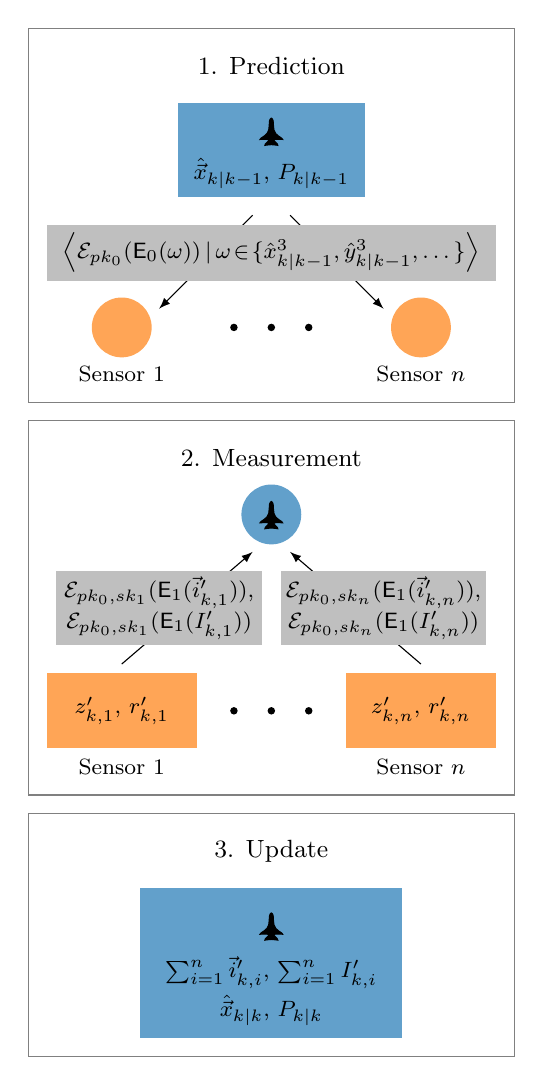
\begin{tikzpicture}[font=\footnotesize,scale=0.95]
    % Prediction
    \draw [gray] (0,3) rectangle (6.5,8);
    \node at (3.25,7.5) {\small 1. Prediction};

    % Navigator
    \fill  [pyplotblue!70] (2,7) rectangle (4.5,5.75);
    \pic[xscale=0.22,yscale=0.3] at (3.25,6.7975) {plane};
    \node at (3.25,6.0625) {$\hat{\vec{x}}_{k|k-1}$, $\mat{P}_{k|k-1}$};
    
    % Sensors
    \fill  (1.25,4) [pyplotorange!70] ellipse (0.4 and 0.4);
    \node at (1.25,3.375) {Sensor $1$};
    \fill  (5.25,4) [pyplotorange!70] ellipse (0.4 and 0.4);
    \node at (5.25,3.375) {Sensor $n$};
        
    \fill [black] (2.75,4) circle (0.05);
    \fill [black] (3.25,4) circle (0.05);
    \fill [black] (3.75,4) circle (0.05);
        
    % Arrows
    \draw [-latex] plot[smooth, tension=.7] coordinates {(3,5.5) (1.75,4.25)};
    \draw [-latex] plot[smooth, tension=.7] coordinates {(3.5,5.5) (4.75,4.25)};
    
    \fill [lightgray]  (0.25,5.375) rectangle (6.25,4.625);
    \node at (3.25,5) {$\left\langle\mathcal{E}_{pk_0}(\mathsf{E}_0(\omega)) \,|\, \omega \!\in\! \{\hat{x}^3_{k|k-1}, \hat{y}^3_{k|k-1}, \dots\}\right\rangle$};
    
    
    % Measurement
    \draw [gray] (0,-2.25) rectangle (6.5,2.75);
    \node at (3.25,2.25) {\small 2. Measurement};
    
    % Navigator
    \fill  (3.25,1.5) [pyplotblue!70] ellipse (0.4 and 0.4);
    \pic[xscale=0.22,yscale=0.3] at (3.25,1.6725) {plane};
        
    % Sensors
    \fill  [pyplotorange!70] (6.25,-1.625)  rectangle (4.25,-0.625);
    \node at (1.25,-1.875) {Sensor $1$};
    \fill  [pyplotorange!70] (2.25,-1.625)  rectangle (0.25,-0.625);
    \node at (5.25,-1.875) {Sensor $n$};
    
    \node at (1.25,-1.125) {$z'_{k,1}$, $r'_{k,1}$};
    \node at (5.25,-1.125) {$z'_{k,n}$, $r'_{k,n}$};
    
    \fill [black] (2.75,-1.125) circle (0.05);
    \fill [black] (3.25,-1.125) circle (0.05);
    \fill [black] (3.75,-1.125) circle (0.05);
    
    % Arrows
    \draw [-latex] plot[smooth, tension=.7] coordinates {(1.25,-0.5) (3,1)};
    \draw [-latex] plot[smooth, tension=.7] coordinates {(5.25,-0.5) (3.5,1)};
    
    \fill [lightgray]  (0.375,0.75) rectangle (3.125,-0.25);
    \node[align=center] at (1.75,0.25) {$\mathcal{E}_{pk_0,sk_1}(\mathsf{E}_1(\vec{i}'_{k,1}))$,\\$\mathcal{E}_{pk_0,sk_1}(\mathsf{E}_1(\mat{I}'_{k,1}))$};
    \fill [lightgray]  (3.375,0.75) rectangle (6.125,-0.25);
    \node[align=center] at (4.75,0.25) {$\mathcal{E}_{pk_0,sk_n}(\mathsf{E}_1(\vec{i}'_{k,n}))$,\\$\mathcal{E}_{pk_0,sk_n}(\mathsf{E}_1(\mat{I}'_{k,n}))$};
    
    
    % Update
    \draw [gray] (0,-5.75) rectangle (6.5,-2.5);
    \node at (3.25,-3) {\small 3. Update};
    
    % Navigator
    \fill  [pyplotblue!70] (1.5,-3.5) rectangle (5,-5.5);
    \pic[xscale=0.22,yscale=0.3] at (3.25,-3.8275) {plane};
    \node at (3.25,-4.625) {$\sum_{i=1}^n \vec{i}'_{k,i}$, $\sum_{i=1}^n\mat{I}'_{k,i}$};
    \node at (3.25,-5.125) {$\hat{\vec{x}}_{k|k}$, $\mat{P}_{k|k}$};
\end{tikzpicture}
\caption{Procedure at timestep $k$ for the proposed privacy-preserving EIF.}
\label{fig:alg_steps}
\end{figure}

% 
% ##       ########    ###    ##    ##    ###     ######   ######## 
% ##       ##         ## ##   ##   ##    ## ##   ##    ##  ##       
% ##       ##        ##   ##  ##  ##    ##   ##  ##        ##       
% ##       ######   ##     ## #####    ##     ## ##   #### ######   
% ##       ##       ######### ##  ##   ######### ##    ##  ##       
% ##       ##       ##     ## ##   ##  ##     ## ##    ##  ##       
% ######## ######## ##     ## ##    ## ##     ##  ######   ######## 
% 

\subsection{Leakage} \label{subsec:leakage}
With the privacy-preserving EIF defined in the previous section, we can now interpret the aggregation leakage of an LCAO scheme in the context of range sensor localisation. The leakage function from the $\mathsf{AggDec}$ algorithm corresponds to the information vector and matrix sums, $\sum_{i=1}^n\vec{i}'_{k,i}$ and $\sum_{i=1}^n\mat{I}'_{k,i}$, respectively. However, recalling that a compromised navigator can learn the individual sums weighted by the same weight, $\{\sum_{i=1}^n2r^{-1}_{k,i},\ \sum_{i=1}^n-r^{-1}_{k,i}s_{x,i},\ \sum_{i=1}^n-2r^{-1}_{k,i}s_{x,i},\ \dots\}$ can be leaked as well. From this leakage, we can see that private sensor information, $z'_{k,i}$, $r'_{k,i}$ and $\vec{s}_i$, is present only in their complete sums
\begin{equation}
    \sum_{i=1}^nz'_{k,i}\,,\ \sum_{i=1}^nr'_{k,i}\,,\ \sum_{i=1}^ns_{x,i}\ \textrm{and}\ \sum_{i=1}^ns_{y,i}\,,\label{eqn:localisation_leakage}
\end{equation}
which in practice correspond to their averages. Therefore, in the context of our proposed localisation method, LCAO leakage corresponds to the averages of sensor private information, while individual sensor information remains private.

% 
%  .d8888b. 8888888 888b     d888 
% d88P  Y88b  888   8888b   d8888 
% Y88b.       888   88888b.d88888 
%  "Y888b.    888   888Y88888P888 
%     "Y88b.  888   888 Y888P 888 
%       "888  888   888  Y8P  888 
% Y88b  d88P  888   888   "   888 
%  "Y8888P" 8888888 888       888 
%                                 
%                                 
%                                 
% 

\section{Simulation and Results} \label{sec:sim_and_results}
As well as having shown the theoretical backing for the security of our scheme, we have simulated the proposed localisation method to evaluate its performance. A two-dimensional, linear, constant velocity process model,
\begin{equation*}
    \vec{x}_{k} = 
    \begin{bmatrix}
        1 & 0 & 0.5 & 0\\
        0 & 1 & 0 & 0.5\\
        0 & 0 & 1 & 0\\
        0 & 0 & 0 & 1
    \end{bmatrix} \cdot \vec{x}_{k-1} + \vec{w}_k\,,
\end{equation*}
where noise term $\vec{w}_k \sim \mathcal{N}(\vec{0}, \mat{Q})$ and
\begin{equation*}
    \mat{Q} = \frac{1}{10^3} \cdot
    \begin{bmatrix}
        0.4 & 0 & 1.3 & 0\\
        0 & 0.4 & 0 & 1.3\\
        1.3 & 0 & 5.0 & 0\\
        0 & 1.3 & 0 & 5.0
    \end{bmatrix}\,,
\end{equation*}
was simulated and tracked with the algorithms in section \ref{subsec:pseudocode}, using a linear Kalman filter for the navigator's local state prediction. Code was written in the C programming language using the MPI library \cite{theopenmpiprojectOpenMPI2020} to support asynchronous computations by the sensors and navigator. The MG1 mask generation function and the SHA256 hash function, from the OpenSSL library \cite{theopensslprojectOpenSSL2020}, were used to implement the required hash function $H$, and the Libpaillier library \cite{bethencourtLibpaillier2010} was used for the Paillier encryption scheme. Additionally, GNU libraries, GSL \cite{thegsldevelopmentteamGSLGNUScientific2019} and GMP \cite{granlundGMPGNUMultiple2020}, were used for algebraic operations and multiple-precision encoded integers, respectively. All execution was performed on a 3.33GHz Xeon W3680 CPU, running on the Windows Subsystem for Linux (WSL).

We have considered multiple sensor layouts, each with four sensors, to capture the dependence of estimated modified measurement variances $r'_{k,i}$ on the original measurements $z_{k,i}$. These layouts of varying sensor distances are shown next to the simulation initial state and a sample track in figure \ref{fig:sim_layouts}.
\begin{figure}[htbp]
    \centering
    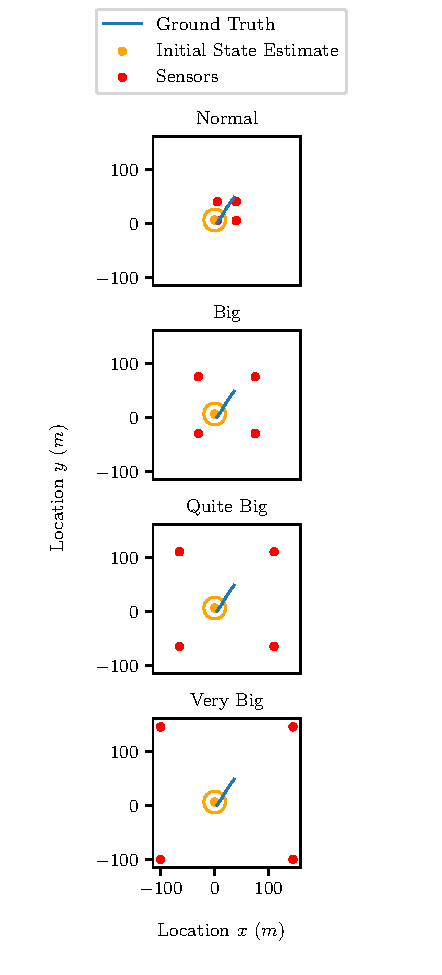
\includegraphics{images/layouts.pdf}
    \caption{Different simulation layouts with varying distances between navigator and sensors.}
    \label{fig:sim_layouts}
\end{figure}
To demonstrate the accuracy of the method, we have compared the root mean square error (RMSE) of the privacy-preserving filter to the standard EIF using unmodified measurements, which is algebraically equivalent to the EKF typically used in industry for linearising non-linear state estimation. Estimation in each layout from figure \ref{fig:sim_layouts} consisted of $50$ filter iterations and was run $1000$ times. Unmodified measurement variances were taken as $r_{k,i}=5$ for all $k>0$ and a large fractional precision factor, $\phi=2^{32}$, was chosen. The results can be seen in figure \ref{fig:sim_layout_errors}.
\begin{figure}[htbp]
    \centering
    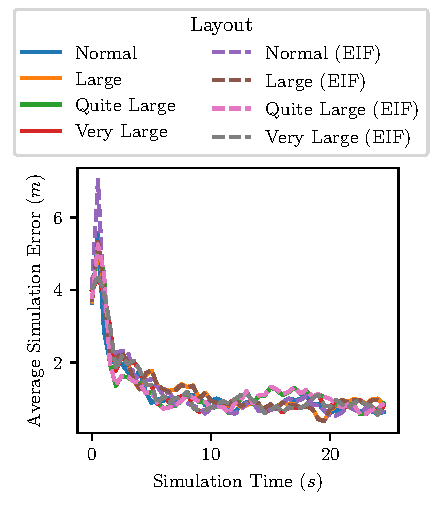
\includegraphics{images/layout_errors.pdf}
    \caption{Average RMSE of our privacy-preserving filter and the standard EIF for different layouts.}
    \vspace{-\baselineskip}
    \label{fig:sim_layout_errors}
\end{figure}
From these results, we can see a strong similarity in filter performance between the privacy-preserving method and that of the traditional EIF. We can also see that the varying average distances between sensors and the navigator have little impact on the differences in performance. We attribute this similarity in RMSE to the conservativeness of estimated modified measurement variances $r'_{k,i}$, resulting in few additional filter divergences, and to the high fractional precision factor, keeping computations consistent with the floating-point arithmetic of the EIF.

In addition to filter error, computational performance is important to consider when relying on cryptographic methods. Figure \ref{fig:sim_timing} shows the averages of $10$ execution times when varying the numbers of sensors and key sizes (bit lengths of $N$). Here, increasing the number of sensors primarily affected the number of inter-process communications and aggregation modular multiplications due to the asynchronous implementation.
\begin{figure}[htbp]
    \centering
    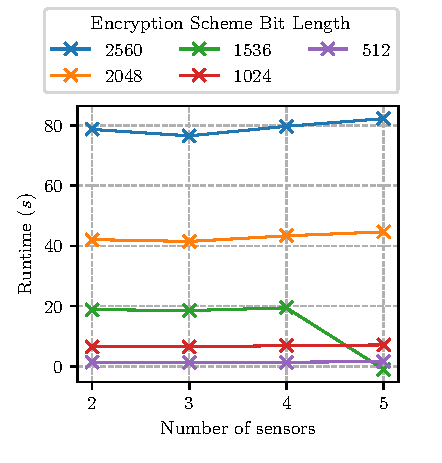
\includegraphics{images/timing.pdf}
    \caption{Runtimes for varying key sizes and numbers of sensors.}
    \label{fig:sim_timing}
\end{figure}
We can see from the figure that the predominant computational costs stem from cryptographic computations and are directly dependent on the chosen key size. The key size should be chosen such that sufficient security is achieved, and the current recommendation, when relying on the DCRA for security (difficulty of factorising $N$), is the use of $2048$ bit length keys \cite{barkerRecommendationPairwiseKey2019}. For our implementation of the filter, run on the aforementioned hardware, this results in a filter update computation duration of roughly $1.7s$.

% 
%  .d8888b.   .d88888b.  888b    888  .d8888b.  
% d88P  Y88b d88P" "Y88b 8888b   888 d88P  Y88b 
% 888    888 888     888 88888b  888 888    888 
% 888        888     888 888Y88b 888 888        
% 888        888     888 888 Y88b888 888        
% 888    888 888     888 888  Y88888 888    888 
% Y88b  d88P Y88b. .d88P 888   Y8888 Y88b  d88P 
%  "Y8888P"   "Y88888P"  888    Y888  "Y8888P"  
%                                               
%                                               
%                                               
% 

\section{Conclusion} \label{sec:conclusion}
We have presented a localisation filter in the presence of range-only sensors, which preserves both navigator and sensor privacies. A suitable cryptographic scheme has been introduced and a filter implementation compared and evaluated. Privacy-preserving range-only localisation is suitable for use in environments where sensor networks are untrusted or location is considered private and we hope to extend the method to broader measurement models in the future. Additional future work includes exploring more computationally efficient encryption schemes and filter reformulations to decrease the filter update duration, exploring the possible security implications of sensors that are not only honest-but-curious and expanding the LCAO notion to guarantee that consistent broadcasts are always made by the navigator.

% 
%        d8888 8888888b.  8888888b.  8888888888 888b    888 8888888b. 8888888 Y88b   d88P 
%       d88888 888   Y88b 888   Y88b 888        8888b   888 888  "Y88b  888    Y88b d88P  
%      d88P888 888    888 888    888 888        88888b  888 888    888  888     Y88o88P   
%     d88P 888 888   d88P 888   d88P 8888888    888Y88b 888 888    888  888      Y888P    
%    d88P  888 8888888P"  8888888P"  888        888 Y88b888 888    888  888      d888b    
%   d88P   888 888        888        888        888  Y88888 888    888  888     d88888b   
%  d8888888888 888        888        888        888   Y8888 888  .d88P  888    d88P Y88b  
% d88P     888 888        888        8888888888 888    Y888 8888888P" 8888888 d88P   Y88b 
%                                                                                         
%                                                                                         
%                                                                                         
% 

\appendices
\section{Linear Combination Aggregator Oblivousness (LCAO)} \label{app:lcao}
The following game between attacker and challenger defines the security notion of LCAO.
\begin{LaTeXdescription}
    \item[Setup] The challenger chooses security parameter $\kappa$, runs the $\mathsf{Setup}(\kappa)$ algorithm and gives $\mathsf{pub}$, $m$ and $pk_0$ to the attacker
    \item[Queries] The attacker can now perform encryptions or submit queries that are answered by the challenger. The types of actions are:
    \begin{LaTeXenumerate}
        \item \textit{Encryption:} The attacker chooses a value $x$ and computes an encryption of $x$ under the aggregator's public key $pk_0$, obtaining $\mathcal{E}_{pk_0}(x)$.
        \item \textit{Weight Queries:} The attacker chooses an instance $t$ and receives the weights for that instance encrypted with the aggregator's public key, $\mathcal{E}_{pk_0}(\omega^{(t)}_{j}),\,j\in\{1,\dots,m\}$.
        \item \textit{Combine Queries:} The attacker chooses a tuple $(i,t,a^{(t)}_{i,1},\dots,a^{(t)}_{i,m})$ such that for any two chosen combine query tuples $(i,t,a^{(t)}_{i,1},\dots,a^{(t)}_{i,m})$ and $(i',t',a^{\prime(t')}_{i',1},\dots,a^{\prime(t')}_{i',m})$, the following condition holds:
        \begin{equation*}
            i = i' \wedge t = t' \implies a^{(t)}_{i,j} = a^{\prime(t')}_{i',j},\,j\in\{1,\dots,m\}\,.
        \end{equation*}
        The attacker is then given back the encryption of the linear combination $\mathcal{E}_{pk_0,sk_i}(\sum^m_{j=1}a^{(t)}_{i,j}\omega^{(t)}_j)$ encrypted under both the aggregator public key $pk_0$ and the secret key $sk_i$.
        \item \textit{Compromise queries:} The attacker chooses $i$ and receives the secret key $sk_i$. The aggregator's secret key may also be compromised (when choosing $i=0$).
    \end{LaTeXenumerate} 
    \item[Challenge] Next, the attacker chooses an instance $t^*$, and a subset of users $S \subseteq U$ where $U$ is the complete set of users for which no combine queries, for the instance $t^*$, and no compromise queries, are made for the duration of the game. The attacker then chooses two series of tuples
    \begin{equation*}
        \left\langle\left(i,t^*,a^{(t^*)(0)}_{i,1},\dots,a^{(t^*)(0)}_{i,m}\right)\,\middle|\,i \in S\right\rangle
    \end{equation*}
    and
    \begin{equation*}
        \left\langle\left(i,t^*,a^{(t^*)(1)}_{i,1},\dots,a^{(t^*)(1)}_{i,m}\right)\,\middle|\, i \in S\right\rangle\,,
    \end{equation*}
    and gives them to the challenger. In the case that $0 \in S$ (\textit{i.e.}, the aggregator is compromised) and $S = U$, it is additionally required that
    \begin{equation*}
        \sum_{i\in S}\sum^{m}_{j=1} a^{(t^*)(0)}_{i,j}\omega^{(t^*)}_j = \sum_{i \in S}\sum^{m}_{j=1} a^{(t^*)(1)}_{i,j}\omega^{(t^*)}_j\,,
    \end{equation*}
    for weights $\omega^{(t^*)}_j,\,j\in\{1,\dots,m\}$ returned by a \textit{Weight Query} with chosen instance $t^*$. The challenger then chooses a random bit $b \in \{1,0\}$ and returns encryptions 
    \begin{equation*}
        \left\langle\mathcal{E}_{pk_0,sk_i}\left(\sum^m_{j=1}a^{(t^*)(b)}_{i,j}\omega^{(t^*)}_j\right)\,\middle|\,i\in S\right\rangle\,.
    \end{equation*}
    \item[More Queries] The attacker can now perform more encryptions and submit queries, so long as the queries do not break the requirements in the Challenge stage. That is, $S \subseteq U$.
    \item[Guess] At the end, the attacker outputs a bit $b'$ and wins the game if and only if $b' = b$. The advantage of an attacker $\mathcal{A}$ is defined as
    \begin{equation*}
        \mathsf{Adv}^{LCAO}(\mathcal{A}) \coloneqq \left\lvert \Pr [b'=b] - \frac{1}{2}\right\rvert\,.
    \end{equation*} 
\end{LaTeXdescription}

\begin{definition}
    An encryption scheme meets LCAO security if no probabilistic adversary, running in polynomial-time with respect to security parameter $\kappa$, has more than a negligible advantage in winning the above security game. That is, for all adversaries $\mathcal{A}$, there exists a negligible function $\eta$, such that
    \begin{equation*}
        \mathsf{Adv}^{LCAO}(\mathcal{A}) \leq \eta(\kappa)\,,
    \end{equation*}
    with probabilities taken over randomness introduced by $\mathcal{A}$, and in $\mathsf{Setup}$, $\mathsf{Enc}$ and $\mathsf{CombEnc}$.
\end{definition}

\section{LCAO Scheme Proof} \label{app:proof}
The scheme in section \ref{sec:lcao_scheme} will be shown to meet LCAO by contrapositive. We show that for any adversary $\mathcal{A}$ playing against a challenger using the scheme, we can always create an adversary $\mathcal{A}'$ playing against a challenger $\mathcal{C}$ using the Joye-Libert scheme, such that
\begin{equation*}
    \mathsf{Adv}^{LCAO}(\mathcal{A}) > \eta_1(\kappa) \implies \mathsf{Adv}^{AO}(\mathcal{A}') > \eta_2(\kappa)\,,
\end{equation*}
for \textit{any} negligible functions $\eta_1$, $\eta_2$ and security parameter $\kappa$. That is, if we assume our scheme is not LCAO secure, then the Joye-Libert scheme is not AO secure (which is not the case, \cite{joyeScalableSchemePrivacyPreserving2013}).
\begin{proof}
    Consider adversary $\mathcal{A}$ playing the LCAO game. The following is a construction of an adversary $\mathcal{A}'$ playing the AO game \cite{shiPrivacyPreservingAggregationTimeSeries2011} against a challenger $\mathcal{C}$ using the Joye-Libert aggregation scheme.
    \begin{LaTeXdescription}
        \item[Setup] When receiving $N$ and $H$ as public parameters from $\mathcal{C}$, choose an $m>1$ and give public parameter $H$, number of weights $m$, and $pk_0=N$ to $\mathcal{A}$.
        \item[Queries] Handle queries from $\mathcal{A}$:
        \begin{LaTeXdescription}
            \item[\textit{Weight Query}] When $\mathcal{A}$ submits a weight query $t$, choose weights $\omega^{(t)}_j,\,j\in\{1,\dots,m\}$ and random values $\rho_j \in \mathbb{Z}_N,\,j\in\{1,\dots,m\}$, and return encryptions 
            \begin{equation*}
                (N+1)^{\omega^{(t)}_{j}}\rho_j^N\pmod{N^2},\,j\in\{1,\dots,m\}
            \end{equation*}
            to $\mathcal{A}$.
            \item[\textit{Combine Query}] When $\mathcal{A}$ submits combine query $(i, t, a^{(t)}_{i,1},\dots,a^{(t)}_{i,m})$, choose weights $\omega^{(t)}_j,j\in\{1,\dots,m\}$ if not already chosen for the instance $t$, and make an AO encryption query $(i, t, \sum^m_{j=1}a^{(t)}_{i,j}\omega^{(t)}_j)$ to $\mathcal{C}$. The received response will be of the form $(N+1)^{\sum^m_{j=1}a^{(t)}_{i,j}\omega^{(t)}_j}H(t)^{sk_i}$; multiply it by $\rho^N$ for a random $\rho \in \mathbb{Z}_N$ and return 
            \begin{equation*}
                (N+1)^{\sum^m_{j=1}a^{(t)}_{i,j}\omega^{(t)}_j}\rho^N H(t)^{sk_i} \pmod{N^2}
            \end{equation*}
            to $\mathcal{A}$.
            \item[\textit{Compromise Query}] When $\mathcal{A}$ submits compromise query $i$, make the same compromise query $i$ to $\mathcal{C}$, and return the recieved secret key $sk_i$ to $\mathcal{A}$.
        \end{LaTeXdescription}
        \item[Challenge] When $\mathcal{A}$ submits challenge series
        \begin{equation*}
            \left\langle\left(i,t^*,a^{(t^*)(0)}_{i,1},\dots,a^{(t^*)(0)}_{i,m}\right)\,\middle|\,i \in S\right\rangle
        \end{equation*}
        and
        \begin{equation*}
            \left\langle\left(i,t^*,a^{(t^*)(1)}_{i,1},\dots,a^{(t^*)(1)}_{i,m}\right)\,\middle|\, i \in S\right\rangle\,,
        \end{equation*}
        choose weights $\omega^{(t^*)}_j,j\in\{1,\dots,m\}$ for instance $t^*$ and submit AO challenge series
        \begin{equation*}
            \left\langle\left(i,t^*,\sum^m_{j=1}a^{(t^*)(0)}_{i,j}\omega^{(t^*)}_j\right)\,\middle|\,i \in S\right\rangle
        \end{equation*}
        and
        \begin{equation*}
            \left\langle\left(i,t^*,\sum^m_{j=1}a^{(t^*)(1)}_{i,j}\omega^{(t^*)}_j\right)\,\middle|\,i \in S\right\rangle\,,
        \end{equation*}
        to $\mathcal{C}$. The received response will be of the form 
        \begin{equation*}
            \left\langle(N+1)^{\sum^m_{j=1}a^{(t^*)(b)}_{i,j}\omega^{(t^*)}_j}H(t^*)^{sk_i}\,\middle|\,i\in U\right\rangle\,,
        \end{equation*}
        for an unknown $b \in \{0,1\}$. Multiply series elements by $\rho_i^N,\,i\in\{1,\dots,n\}$ for randomly chosen $\rho_i \in \mathbb{Z}_N$ and return
        \begin{equation*}
            \left\langle(N+1)^{\sum^m_{j=1}a^{(t^*)(b)}_{i,j}\omega^{(t^*)}_j}\rho_i^N H(t^*)^{sk_i}\,\middle|\,i\in U\right\rangle
        \end{equation*}
        to $\mathcal{A}$.
        \item[Guess] When $\mathcal{A}$ makes guess $b'$, make the same guess $b'$ to~$\mathcal{C}$.
    \end{LaTeXdescription}

    In the above construction, $\mathcal{C}$ follows the Joye-Libert scheme exactly, and to $\mathcal{A}$, $\mathcal{A}'$ follows the scheme in section \ref{sec:lcao_scheme} exactly. Since $\mathcal{A}'$ runs in polynomial-time to security parameter when $\mathcal{A}$ does, and no non-negligible advantage adversary to $\mathcal{C}$ exists, we conclude that no non-negligible advantage adversary $\mathcal{A}$ exists. That is, there exists a negligible function $\eta$, such that
    \begin{equation*}
        \mathsf{Adv}^{LCAO}(\mathcal{A}) \leq \eta(\kappa)
    \end{equation*}
    for security parameter $\kappa$. Lastly, the function $H$ used by our scheme is treated as a random oracle in the Joye-Libert AO proof and will, therefore, prove our scheme secure in the random oracle model as well.
\end{proof}


% Can use something like this to put references on a page
% by themselves when using endfloat and the captionsoff option.
\ifCLASSOPTIONcaptionsoff
  \newpage
\fi


\bibliographystyle{IEEEtranBST/IEEEtran}
\bibliography{BibTeX/PrivateEIFLocalisation}

% 
% 888888b.  8888888 .d88888b.   .d8888b.  
% 888  "88b   888  d88P" "Y88b d88P  Y88b 
% 888  .88P   888  888     888 Y88b.      
% 8888888K.   888  888     888  "Y888b.   
% 888  "Y88b  888  888     888     "Y88b. 
% 888    888  888  888     888       "888 
% 888   d88P  888  Y88b. .d88P Y88b  d88P 
% 8888888P" 8888888 "Y88888P"   "Y8888P"  
%                                         
%                                         
%                                         
% 

%\vspace{-1\baselineskip}
\begin{IEEEbiography}[{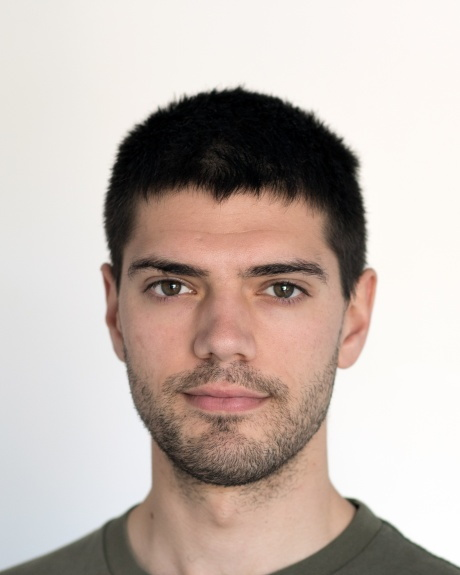
\includegraphics[width=1in,height=1.25in,clip,keepaspectratio]{images/marko_ristic}}]{Marko Ristic}
received his software engineering diploma in 2018 at the University of Melbourne, Australia. In 2019, he began work as a researcher at the Intelligent Sensor-Actuator-Systems Laboratory, Karlsruhe Institute of Technology (KIT), Germany, and since 2021, he has been pursuing a Ph.D. at the Autonomous Multisensor Systems (AMS) group, Otto von Guericke University, Germany. His research interests include encrypted and privacy-preserving signal processing, focusing on state estimation, sensor fusion, and distributed localisation.
\end{IEEEbiography}

%\vspace{-1\baselineskip}
\begin{IEEEbiography}[{
\includegraphics[width=1in,height=1.25in,clip,keepaspectratio]{images/benjamin_noack}}]{Benjamin Noack}
is a professor of Computer Science at the Otto von Guericke University Magdeburg in Germany and head of the Autonomous Multisensor Systems (AMS) group. He received his diploma in computer science from the Karlsruhe Institute of Technology (KIT), Germany, in 2009. Afterward, he obtained his Ph.D. in 2013 at the Intelligent Sensor–Actuator-Systems Laboratory, Karlsruhe Institute of Technology (KIT), Germany. His research interests are in the areas of multi-sensor data fusion, distributed and decentralized Kalman filtering, combined stochastic and set-membership approaches to state estimation, and event-based systems.
\end{IEEEbiography}

%\vspace{-1\baselineskip}
\begin{IEEEbiography}[{
\includegraphics[width=1in,height=1.25in,clip,keepaspectratio]{images/uwe_d_hanebeck}}]{Uwe D. Hanebeck}
is a chaired professor of Computer Science at the Karlsruhe Institute of Technology (KIT) in Germany and director of the Intelligent Sensor–Actuator-Systems Laboratory (ISAS). He obtained his Ph.D. degree in 1997 and his habilitation degree in 2003, both in Electrical Engineering from the Technical University in Munich, Germany. His research interests are in the areas of information fusion, nonlinear state estimation, stochastic modeling, system identification, and control with a strong emphasis on theory-driven approaches based on stochastic system theory and uncertainty models. He is author and coauthor of more than 500 publications in various high-ranking journals and conferences and an IEEE Fellow.
\end{IEEEbiography}

% You can push biographies down or up by placing
% a \vfill before or after them. The appropriate
% use of \vfill depends on what kind of text is
% on the last page and whether or not the columns
% are being equalized.

%\vfill

% Can be used to pull up biographies so that the bottom of the last one
% is flush with the other column.
%\enlargethispage{-5in}

% that's all folks
\end{document}
